% Project report built on the official AISR Overleaf template (main.tex).
% Preamble, title page, border, fonts, margins, Index and page numbering are kept
% exactly as in the template; only the content changes.
% Build:  make report   (pdflatex twice, from this folder)
% The logo upes_logo.png comes from AISR_Sample_Project_Report_Overleaf.zip (kept local).
\documentclass[12pt,a4paper]{article}
\usepackage[T1]{fontenc}
\usepackage{newtxtext,newtxmath}
\usepackage[left=3cm,right=2.5cm,top=2.5cm,bottom=2.5cm,footskip=0.75cm]{geometry}
\usepackage{graphicx,calc}
\usepackage{setspace,eso-pic,tikz,array,booktabs,longtable,enumitem,caption,titlesec,fancyhdr,tocloft}
\usetikzlibrary{arrows.meta,positioning,shapes.geometric,calc}
\usepackage{amsmath,float,algorithm,algpseudocode}
\usepackage[hidelinks]{hyperref}
\onehalfspacing
\setlength{\parindent}{0pt}\setlength{\parskip}{6pt}

% single-line page border on every page (title page included)
\AddToShipoutPictureBG{%
  \AtPageLowerLeft{\put(\LenToUnit{1.5cm},\LenToUnit{1.5cm}){%
    \framebox(\LenToUnit{\paperwidth-3cm},\LenToUnit{\paperheight-3cm}){}}}}
\setlength{\fboxrule}{0.8pt}

\titleformat{\section}{\fontsize{14}{17}\bfseries}{\thesection.}{0.6em}{}
\titleformat{\subsection}{\normalsize\bfseries}{\thesubsection}{0.6em}{}
\titlespacing*{\section}{0pt}{12pt}{6pt}
\captionsetup{font=small,labelfont=bf}
\fancypagestyle{plain}{\fancyhf{}\fancyfoot[C]{\thepage}\renewcommand{\headrulewidth}{0pt}}
\pagestyle{plain}
\renewcommand{\cftsecleader}{\cftdotfill{\cftdotsep}}
\renewcommand{\contentsname}{Index}
\newcolumntype{P}[1]{>{\raggedright\arraybackslash}p{#1}}
\newcommand{\note}[1]{\textit{[#1]}}
\graphicspath{{../results/figures/}}

% every result number comes from results/summary.csv through these macros
% Generated by analysis/tables.py from results/summary.csv - do not edit.
\providecommand{\R}[3]{\csname R:#1:#2:#3\endcsname}
\expandafter\def\csname R:E1:baseline:runs\endcsname{1}
\expandafter\def\csname R:E1:baseline:success_count\endcsname{1}
\expandafter\def\csname R:E1:baseline:crash_count\endcsname{0}
\expandafter\def\csname R:E1:baseline:path_rmse_m\endcsname{--}
\expandafter\def\csname R:E1:baseline:mean_path_rmse_m\endcsname{--}
\expandafter\def\csname R:E1:baseline:std_path_rmse_m\endcsname{0.000}
\expandafter\def\csname R:E1:baseline:path_max_err_m\endcsname{--}
\expandafter\def\csname R:E1:baseline:mean_path_max_err_m\endcsname{--}
\expandafter\def\csname R:E1:baseline:std_path_max_err_m\endcsname{0.000}
\expandafter\def\csname R:E1:baseline:mission_time_s\endcsname{--}
\expandafter\def\csname R:E1:baseline:mean_mission_time_s\endcsname{--}
\expandafter\def\csname R:E1:baseline:std_mission_time_s\endcsname{0.0}
\expandafter\def\csname R:E1:baseline:max_tilt_deg\endcsname{2.1}
\expandafter\def\csname R:E1:baseline:mean_max_tilt_deg\endcsname{2.1}
\expandafter\def\csname R:E1:baseline:std_max_tilt_deg\endcsname{0.0}
\expandafter\def\csname R:E1:baseline:control_effort\endcsname{51.1}
\expandafter\def\csname R:E1:baseline:mean_control_effort\endcsname{51.1}
\expandafter\def\csname R:E1:baseline:std_control_effort\endcsname{0.0}
\expandafter\def\csname R:E1:baseline:waypoints_reached\endcsname{--}
\expandafter\def\csname R:E1:baseline:mean_waypoints_reached\endcsname{--}
\expandafter\def\csname R:E1:baseline:std_waypoints_reached\endcsname{0}
\expandafter\def\csname R:E1:baseline:step1_rise_time_s\endcsname{1.50}
\expandafter\def\csname R:E1:baseline:mean_step1_rise_time_s\endcsname{1.50}
\expandafter\def\csname R:E1:baseline:std_step1_rise_time_s\endcsname{0.00}
\expandafter\def\csname R:E1:baseline:step1_overshoot_pct\endcsname{0.0}
\expandafter\def\csname R:E1:baseline:mean_step1_overshoot_pct\endcsname{0.0}
\expandafter\def\csname R:E1:baseline:std_step1_overshoot_pct\endcsname{0.0}
\expandafter\def\csname R:E1:baseline:step1_settling_time_s\endcsname{--}
\expandafter\def\csname R:E1:baseline:mean_step1_settling_time_s\endcsname{--}
\expandafter\def\csname R:E1:baseline:std_step1_settling_time_s\endcsname{0.0}
\expandafter\def\csname R:E1:baseline:step1_ss_error_m\endcsname{0.054}
\expandafter\def\csname R:E1:baseline:mean_step1_ss_error_m\endcsname{0.054}
\expandafter\def\csname R:E1:baseline:std_step1_ss_error_m\endcsname{0.000}
\expandafter\def\csname R:E1:baseline:step2_rise_time_s\endcsname{1.30}
\expandafter\def\csname R:E1:baseline:mean_step2_rise_time_s\endcsname{1.30}
\expandafter\def\csname R:E1:baseline:std_step2_rise_time_s\endcsname{0.00}
\expandafter\def\csname R:E1:baseline:step2_overshoot_pct\endcsname{6.2}
\expandafter\def\csname R:E1:baseline:mean_step2_overshoot_pct\endcsname{6.2}
\expandafter\def\csname R:E1:baseline:std_step2_overshoot_pct\endcsname{0.0}
\expandafter\def\csname R:E1:baseline:step2_settling_time_s\endcsname{--}
\expandafter\def\csname R:E1:baseline:mean_step2_settling_time_s\endcsname{--}
\expandafter\def\csname R:E1:baseline:std_step2_settling_time_s\endcsname{0.0}
\expandafter\def\csname R:E1:baseline:step2_ss_error_m\endcsname{0.054}
\expandafter\def\csname R:E1:baseline:mean_step2_ss_error_m\endcsname{0.054}
\expandafter\def\csname R:E1:baseline:std_step2_ss_error_m\endcsname{0.000}
\expandafter\def\csname R:E1:improved:runs\endcsname{1}
\expandafter\def\csname R:E1:improved:success_count\endcsname{1}
\expandafter\def\csname R:E1:improved:crash_count\endcsname{0}
\expandafter\def\csname R:E1:improved:path_rmse_m\endcsname{--}
\expandafter\def\csname R:E1:improved:mean_path_rmse_m\endcsname{--}
\expandafter\def\csname R:E1:improved:std_path_rmse_m\endcsname{0.000}
\expandafter\def\csname R:E1:improved:path_max_err_m\endcsname{--}
\expandafter\def\csname R:E1:improved:mean_path_max_err_m\endcsname{--}
\expandafter\def\csname R:E1:improved:std_path_max_err_m\endcsname{0.000}
\expandafter\def\csname R:E1:improved:mission_time_s\endcsname{--}
\expandafter\def\csname R:E1:improved:mean_mission_time_s\endcsname{--}
\expandafter\def\csname R:E1:improved:std_mission_time_s\endcsname{0.0}
\expandafter\def\csname R:E1:improved:max_tilt_deg\endcsname{0.9}
\expandafter\def\csname R:E1:improved:mean_max_tilt_deg\endcsname{0.9}
\expandafter\def\csname R:E1:improved:std_max_tilt_deg\endcsname{0.0}
\expandafter\def\csname R:E1:improved:control_effort\endcsname{20.4}
\expandafter\def\csname R:E1:improved:mean_control_effort\endcsname{20.4}
\expandafter\def\csname R:E1:improved:std_control_effort\endcsname{0.0}
\expandafter\def\csname R:E1:improved:waypoints_reached\endcsname{--}
\expandafter\def\csname R:E1:improved:mean_waypoints_reached\endcsname{--}
\expandafter\def\csname R:E1:improved:std_waypoints_reached\endcsname{0}
\expandafter\def\csname R:E1:improved:step1_rise_time_s\endcsname{2.41}
\expandafter\def\csname R:E1:improved:mean_step1_rise_time_s\endcsname{2.41}
\expandafter\def\csname R:E1:improved:std_step1_rise_time_s\endcsname{0.00}
\expandafter\def\csname R:E1:improved:step1_overshoot_pct\endcsname{1.3}
\expandafter\def\csname R:E1:improved:mean_step1_overshoot_pct\endcsname{1.3}
\expandafter\def\csname R:E1:improved:std_step1_overshoot_pct\endcsname{0.0}
\expandafter\def\csname R:E1:improved:step1_settling_time_s\endcsname{6.2}
\expandafter\def\csname R:E1:improved:mean_step1_settling_time_s\endcsname{6.2}
\expandafter\def\csname R:E1:improved:std_step1_settling_time_s\endcsname{0.0}
\expandafter\def\csname R:E1:improved:step1_ss_error_m\endcsname{0.005}
\expandafter\def\csname R:E1:improved:mean_step1_ss_error_m\endcsname{0.005}
\expandafter\def\csname R:E1:improved:std_step1_ss_error_m\endcsname{0.000}
\expandafter\def\csname R:E1:improved:step2_rise_time_s\endcsname{1.50}
\expandafter\def\csname R:E1:improved:mean_step2_rise_time_s\endcsname{1.50}
\expandafter\def\csname R:E1:improved:std_step2_rise_time_s\endcsname{0.00}
\expandafter\def\csname R:E1:improved:step2_overshoot_pct\endcsname{2.9}
\expandafter\def\csname R:E1:improved:mean_step2_overshoot_pct\endcsname{2.9}
\expandafter\def\csname R:E1:improved:std_step2_overshoot_pct\endcsname{0.0}
\expandafter\def\csname R:E1:improved:step2_settling_time_s\endcsname{6.1}
\expandafter\def\csname R:E1:improved:mean_step2_settling_time_s\endcsname{6.1}
\expandafter\def\csname R:E1:improved:std_step2_settling_time_s\endcsname{0.0}
\expandafter\def\csname R:E1:improved:step2_ss_error_m\endcsname{0.003}
\expandafter\def\csname R:E1:improved:mean_step2_ss_error_m\endcsname{0.003}
\expandafter\def\csname R:E1:improved:std_step2_ss_error_m\endcsname{0.000}
\expandafter\def\csname R:E2:baseline:runs\endcsname{1}
\expandafter\def\csname R:E2:baseline:success_count\endcsname{1}
\expandafter\def\csname R:E2:baseline:crash_count\endcsname{0}
\expandafter\def\csname R:E2:baseline:path_rmse_m\endcsname{0.063}
\expandafter\def\csname R:E2:baseline:mean_path_rmse_m\endcsname{0.063}
\expandafter\def\csname R:E2:baseline:std_path_rmse_m\endcsname{0.000}
\expandafter\def\csname R:E2:baseline:path_max_err_m\endcsname{0.109}
\expandafter\def\csname R:E2:baseline:mean_path_max_err_m\endcsname{0.109}
\expandafter\def\csname R:E2:baseline:std_path_max_err_m\endcsname{0.000}
\expandafter\def\csname R:E2:baseline:mission_time_s\endcsname{20.8}
\expandafter\def\csname R:E2:baseline:mean_mission_time_s\endcsname{20.8}
\expandafter\def\csname R:E2:baseline:std_mission_time_s\endcsname{0.0}
\expandafter\def\csname R:E2:baseline:max_tilt_deg\endcsname{11.8}
\expandafter\def\csname R:E2:baseline:mean_max_tilt_deg\endcsname{11.8}
\expandafter\def\csname R:E2:baseline:std_max_tilt_deg\endcsname{0.0}
\expandafter\def\csname R:E2:baseline:control_effort\endcsname{27.1}
\expandafter\def\csname R:E2:baseline:mean_control_effort\endcsname{27.1}
\expandafter\def\csname R:E2:baseline:std_control_effort\endcsname{0.0}
\expandafter\def\csname R:E2:baseline:waypoints_reached\endcsname{5}
\expandafter\def\csname R:E2:baseline:mean_waypoints_reached\endcsname{5}
\expandafter\def\csname R:E2:baseline:std_waypoints_reached\endcsname{0}
\expandafter\def\csname R:E2:baseline:step1_rise_time_s\endcsname{--}
\expandafter\def\csname R:E2:baseline:mean_step1_rise_time_s\endcsname{--}
\expandafter\def\csname R:E2:baseline:std_step1_rise_time_s\endcsname{0.00}
\expandafter\def\csname R:E2:baseline:step1_overshoot_pct\endcsname{--}
\expandafter\def\csname R:E2:baseline:mean_step1_overshoot_pct\endcsname{--}
\expandafter\def\csname R:E2:baseline:std_step1_overshoot_pct\endcsname{0.0}
\expandafter\def\csname R:E2:baseline:step1_settling_time_s\endcsname{--}
\expandafter\def\csname R:E2:baseline:mean_step1_settling_time_s\endcsname{--}
\expandafter\def\csname R:E2:baseline:std_step1_settling_time_s\endcsname{0.0}
\expandafter\def\csname R:E2:baseline:step1_ss_error_m\endcsname{--}
\expandafter\def\csname R:E2:baseline:mean_step1_ss_error_m\endcsname{--}
\expandafter\def\csname R:E2:baseline:std_step1_ss_error_m\endcsname{0.000}
\expandafter\def\csname R:E2:baseline:step2_rise_time_s\endcsname{--}
\expandafter\def\csname R:E2:baseline:mean_step2_rise_time_s\endcsname{--}
\expandafter\def\csname R:E2:baseline:std_step2_rise_time_s\endcsname{0.00}
\expandafter\def\csname R:E2:baseline:step2_overshoot_pct\endcsname{--}
\expandafter\def\csname R:E2:baseline:mean_step2_overshoot_pct\endcsname{--}
\expandafter\def\csname R:E2:baseline:std_step2_overshoot_pct\endcsname{0.0}
\expandafter\def\csname R:E2:baseline:step2_settling_time_s\endcsname{--}
\expandafter\def\csname R:E2:baseline:mean_step2_settling_time_s\endcsname{--}
\expandafter\def\csname R:E2:baseline:std_step2_settling_time_s\endcsname{0.0}
\expandafter\def\csname R:E2:baseline:step2_ss_error_m\endcsname{--}
\expandafter\def\csname R:E2:baseline:mean_step2_ss_error_m\endcsname{--}
\expandafter\def\csname R:E2:baseline:std_step2_ss_error_m\endcsname{0.000}
\expandafter\def\csname R:E2:improved:runs\endcsname{1}
\expandafter\def\csname R:E2:improved:success_count\endcsname{1}
\expandafter\def\csname R:E2:improved:crash_count\endcsname{0}
\expandafter\def\csname R:E2:improved:path_rmse_m\endcsname{0.049}
\expandafter\def\csname R:E2:improved:mean_path_rmse_m\endcsname{0.049}
\expandafter\def\csname R:E2:improved:std_path_rmse_m\endcsname{0.000}
\expandafter\def\csname R:E2:improved:path_max_err_m\endcsname{0.080}
\expandafter\def\csname R:E2:improved:mean_path_max_err_m\endcsname{0.080}
\expandafter\def\csname R:E2:improved:std_path_max_err_m\endcsname{0.000}
\expandafter\def\csname R:E2:improved:mission_time_s\endcsname{19.2}
\expandafter\def\csname R:E2:improved:mean_mission_time_s\endcsname{19.2}
\expandafter\def\csname R:E2:improved:std_mission_time_s\endcsname{0.0}
\expandafter\def\csname R:E2:improved:max_tilt_deg\endcsname{8.2}
\expandafter\def\csname R:E2:improved:mean_max_tilt_deg\endcsname{8.2}
\expandafter\def\csname R:E2:improved:std_max_tilt_deg\endcsname{0.0}
\expandafter\def\csname R:E2:improved:control_effort\endcsname{12.1}
\expandafter\def\csname R:E2:improved:mean_control_effort\endcsname{12.1}
\expandafter\def\csname R:E2:improved:std_control_effort\endcsname{0.0}
\expandafter\def\csname R:E2:improved:waypoints_reached\endcsname{5}
\expandafter\def\csname R:E2:improved:mean_waypoints_reached\endcsname{5}
\expandafter\def\csname R:E2:improved:std_waypoints_reached\endcsname{0}
\expandafter\def\csname R:E2:improved:step1_rise_time_s\endcsname{--}
\expandafter\def\csname R:E2:improved:mean_step1_rise_time_s\endcsname{--}
\expandafter\def\csname R:E2:improved:std_step1_rise_time_s\endcsname{0.00}
\expandafter\def\csname R:E2:improved:step1_overshoot_pct\endcsname{--}
\expandafter\def\csname R:E2:improved:mean_step1_overshoot_pct\endcsname{--}
\expandafter\def\csname R:E2:improved:std_step1_overshoot_pct\endcsname{0.0}
\expandafter\def\csname R:E2:improved:step1_settling_time_s\endcsname{--}
\expandafter\def\csname R:E2:improved:mean_step1_settling_time_s\endcsname{--}
\expandafter\def\csname R:E2:improved:std_step1_settling_time_s\endcsname{0.0}
\expandafter\def\csname R:E2:improved:step1_ss_error_m\endcsname{--}
\expandafter\def\csname R:E2:improved:mean_step1_ss_error_m\endcsname{--}
\expandafter\def\csname R:E2:improved:std_step1_ss_error_m\endcsname{0.000}
\expandafter\def\csname R:E2:improved:step2_rise_time_s\endcsname{--}
\expandafter\def\csname R:E2:improved:mean_step2_rise_time_s\endcsname{--}
\expandafter\def\csname R:E2:improved:std_step2_rise_time_s\endcsname{0.00}
\expandafter\def\csname R:E2:improved:step2_overshoot_pct\endcsname{--}
\expandafter\def\csname R:E2:improved:mean_step2_overshoot_pct\endcsname{--}
\expandafter\def\csname R:E2:improved:std_step2_overshoot_pct\endcsname{0.0}
\expandafter\def\csname R:E2:improved:step2_settling_time_s\endcsname{--}
\expandafter\def\csname R:E2:improved:mean_step2_settling_time_s\endcsname{--}
\expandafter\def\csname R:E2:improved:std_step2_settling_time_s\endcsname{0.0}
\expandafter\def\csname R:E2:improved:step2_ss_error_m\endcsname{--}
\expandafter\def\csname R:E2:improved:mean_step2_ss_error_m\endcsname{--}
\expandafter\def\csname R:E2:improved:std_step2_ss_error_m\endcsname{0.000}
\expandafter\def\csname R:E3:baseline:runs\endcsname{1}
\expandafter\def\csname R:E3:baseline:success_count\endcsname{1}
\expandafter\def\csname R:E3:baseline:crash_count\endcsname{0}
\expandafter\def\csname R:E3:baseline:path_rmse_m\endcsname{0.275}
\expandafter\def\csname R:E3:baseline:mean_path_rmse_m\endcsname{0.275}
\expandafter\def\csname R:E3:baseline:std_path_rmse_m\endcsname{0.000}
\expandafter\def\csname R:E3:baseline:path_max_err_m\endcsname{0.542}
\expandafter\def\csname R:E3:baseline:mean_path_max_err_m\endcsname{0.542}
\expandafter\def\csname R:E3:baseline:std_path_max_err_m\endcsname{0.000}
\expandafter\def\csname R:E3:baseline:mission_time_s\endcsname{20.4}
\expandafter\def\csname R:E3:baseline:mean_mission_time_s\endcsname{20.4}
\expandafter\def\csname R:E3:baseline:std_mission_time_s\endcsname{0.0}
\expandafter\def\csname R:E3:baseline:max_tilt_deg\endcsname{10.2}
\expandafter\def\csname R:E3:baseline:mean_max_tilt_deg\endcsname{10.2}
\expandafter\def\csname R:E3:baseline:std_max_tilt_deg\endcsname{0.0}
\expandafter\def\csname R:E3:baseline:control_effort\endcsname{35.2}
\expandafter\def\csname R:E3:baseline:mean_control_effort\endcsname{35.2}
\expandafter\def\csname R:E3:baseline:std_control_effort\endcsname{0.0}
\expandafter\def\csname R:E3:baseline:waypoints_reached\endcsname{5}
\expandafter\def\csname R:E3:baseline:mean_waypoints_reached\endcsname{5}
\expandafter\def\csname R:E3:baseline:std_waypoints_reached\endcsname{0}
\expandafter\def\csname R:E3:baseline:step1_rise_time_s\endcsname{--}
\expandafter\def\csname R:E3:baseline:mean_step1_rise_time_s\endcsname{--}
\expandafter\def\csname R:E3:baseline:std_step1_rise_time_s\endcsname{0.00}
\expandafter\def\csname R:E3:baseline:step1_overshoot_pct\endcsname{--}
\expandafter\def\csname R:E3:baseline:mean_step1_overshoot_pct\endcsname{--}
\expandafter\def\csname R:E3:baseline:std_step1_overshoot_pct\endcsname{0.0}
\expandafter\def\csname R:E3:baseline:step1_settling_time_s\endcsname{--}
\expandafter\def\csname R:E3:baseline:mean_step1_settling_time_s\endcsname{--}
\expandafter\def\csname R:E3:baseline:std_step1_settling_time_s\endcsname{0.0}
\expandafter\def\csname R:E3:baseline:step1_ss_error_m\endcsname{--}
\expandafter\def\csname R:E3:baseline:mean_step1_ss_error_m\endcsname{--}
\expandafter\def\csname R:E3:baseline:std_step1_ss_error_m\endcsname{0.000}
\expandafter\def\csname R:E3:baseline:step2_rise_time_s\endcsname{--}
\expandafter\def\csname R:E3:baseline:mean_step2_rise_time_s\endcsname{--}
\expandafter\def\csname R:E3:baseline:std_step2_rise_time_s\endcsname{0.00}
\expandafter\def\csname R:E3:baseline:step2_overshoot_pct\endcsname{--}
\expandafter\def\csname R:E3:baseline:mean_step2_overshoot_pct\endcsname{--}
\expandafter\def\csname R:E3:baseline:std_step2_overshoot_pct\endcsname{0.0}
\expandafter\def\csname R:E3:baseline:step2_settling_time_s\endcsname{--}
\expandafter\def\csname R:E3:baseline:mean_step2_settling_time_s\endcsname{--}
\expandafter\def\csname R:E3:baseline:std_step2_settling_time_s\endcsname{0.0}
\expandafter\def\csname R:E3:baseline:step2_ss_error_m\endcsname{--}
\expandafter\def\csname R:E3:baseline:mean_step2_ss_error_m\endcsname{--}
\expandafter\def\csname R:E3:baseline:std_step2_ss_error_m\endcsname{0.000}
\expandafter\def\csname R:E3:improved:runs\endcsname{1}
\expandafter\def\csname R:E3:improved:success_count\endcsname{1}
\expandafter\def\csname R:E3:improved:crash_count\endcsname{0}
\expandafter\def\csname R:E3:improved:path_rmse_m\endcsname{0.046}
\expandafter\def\csname R:E3:improved:mean_path_rmse_m\endcsname{0.046}
\expandafter\def\csname R:E3:improved:std_path_rmse_m\endcsname{0.000}
\expandafter\def\csname R:E3:improved:path_max_err_m\endcsname{0.068}
\expandafter\def\csname R:E3:improved:mean_path_max_err_m\endcsname{0.068}
\expandafter\def\csname R:E3:improved:std_path_max_err_m\endcsname{0.000}
\expandafter\def\csname R:E3:improved:mission_time_s\endcsname{18.7}
\expandafter\def\csname R:E3:improved:mean_mission_time_s\endcsname{18.7}
\expandafter\def\csname R:E3:improved:std_mission_time_s\endcsname{0.0}
\expandafter\def\csname R:E3:improved:max_tilt_deg\endcsname{7.4}
\expandafter\def\csname R:E3:improved:mean_max_tilt_deg\endcsname{7.4}
\expandafter\def\csname R:E3:improved:std_max_tilt_deg\endcsname{0.0}
\expandafter\def\csname R:E3:improved:control_effort\endcsname{12.6}
\expandafter\def\csname R:E3:improved:mean_control_effort\endcsname{12.6}
\expandafter\def\csname R:E3:improved:std_control_effort\endcsname{0.0}
\expandafter\def\csname R:E3:improved:waypoints_reached\endcsname{5}
\expandafter\def\csname R:E3:improved:mean_waypoints_reached\endcsname{5}
\expandafter\def\csname R:E3:improved:std_waypoints_reached\endcsname{0}
\expandafter\def\csname R:E3:improved:step1_rise_time_s\endcsname{--}
\expandafter\def\csname R:E3:improved:mean_step1_rise_time_s\endcsname{--}
\expandafter\def\csname R:E3:improved:std_step1_rise_time_s\endcsname{0.00}
\expandafter\def\csname R:E3:improved:step1_overshoot_pct\endcsname{--}
\expandafter\def\csname R:E3:improved:mean_step1_overshoot_pct\endcsname{--}
\expandafter\def\csname R:E3:improved:std_step1_overshoot_pct\endcsname{0.0}
\expandafter\def\csname R:E3:improved:step1_settling_time_s\endcsname{--}
\expandafter\def\csname R:E3:improved:mean_step1_settling_time_s\endcsname{--}
\expandafter\def\csname R:E3:improved:std_step1_settling_time_s\endcsname{0.0}
\expandafter\def\csname R:E3:improved:step1_ss_error_m\endcsname{--}
\expandafter\def\csname R:E3:improved:mean_step1_ss_error_m\endcsname{--}
\expandafter\def\csname R:E3:improved:std_step1_ss_error_m\endcsname{0.000}
\expandafter\def\csname R:E3:improved:step2_rise_time_s\endcsname{--}
\expandafter\def\csname R:E3:improved:mean_step2_rise_time_s\endcsname{--}
\expandafter\def\csname R:E3:improved:std_step2_rise_time_s\endcsname{0.00}
\expandafter\def\csname R:E3:improved:step2_overshoot_pct\endcsname{--}
\expandafter\def\csname R:E3:improved:mean_step2_overshoot_pct\endcsname{--}
\expandafter\def\csname R:E3:improved:std_step2_overshoot_pct\endcsname{0.0}
\expandafter\def\csname R:E3:improved:step2_settling_time_s\endcsname{--}
\expandafter\def\csname R:E3:improved:mean_step2_settling_time_s\endcsname{--}
\expandafter\def\csname R:E3:improved:std_step2_settling_time_s\endcsname{0.0}
\expandafter\def\csname R:E3:improved:step2_ss_error_m\endcsname{--}
\expandafter\def\csname R:E3:improved:mean_step2_ss_error_m\endcsname{--}
\expandafter\def\csname R:E3:improved:std_step2_ss_error_m\endcsname{0.000}
\expandafter\def\csname R:E4:baseline:runs\endcsname{1}
\expandafter\def\csname R:E4:baseline:success_count\endcsname{0}
\expandafter\def\csname R:E4:baseline:crash_count\endcsname{0}
\expandafter\def\csname R:E4:baseline:path_rmse_m\endcsname{0.517}
\expandafter\def\csname R:E4:baseline:mean_path_rmse_m\endcsname{0.517}
\expandafter\def\csname R:E4:baseline:std_path_rmse_m\endcsname{0.000}
\expandafter\def\csname R:E4:baseline:path_max_err_m\endcsname{0.650}
\expandafter\def\csname R:E4:baseline:mean_path_max_err_m\endcsname{0.650}
\expandafter\def\csname R:E4:baseline:std_path_max_err_m\endcsname{0.000}
\expandafter\def\csname R:E4:baseline:mission_time_s\endcsname{--}
\expandafter\def\csname R:E4:baseline:mean_mission_time_s\endcsname{--}
\expandafter\def\csname R:E4:baseline:std_mission_time_s\endcsname{0.0}
\expandafter\def\csname R:E4:baseline:max_tilt_deg\endcsname{13.4}
\expandafter\def\csname R:E4:baseline:mean_max_tilt_deg\endcsname{13.4}
\expandafter\def\csname R:E4:baseline:std_max_tilt_deg\endcsname{0.0}
\expandafter\def\csname R:E4:baseline:control_effort\endcsname{24.9}
\expandafter\def\csname R:E4:baseline:mean_control_effort\endcsname{24.9}
\expandafter\def\csname R:E4:baseline:std_control_effort\endcsname{0.0}
\expandafter\def\csname R:E4:baseline:waypoints_reached\endcsname{3}
\expandafter\def\csname R:E4:baseline:mean_waypoints_reached\endcsname{3}
\expandafter\def\csname R:E4:baseline:std_waypoints_reached\endcsname{0}
\expandafter\def\csname R:E4:baseline:step1_rise_time_s\endcsname{--}
\expandafter\def\csname R:E4:baseline:mean_step1_rise_time_s\endcsname{--}
\expandafter\def\csname R:E4:baseline:std_step1_rise_time_s\endcsname{0.00}
\expandafter\def\csname R:E4:baseline:step1_overshoot_pct\endcsname{--}
\expandafter\def\csname R:E4:baseline:mean_step1_overshoot_pct\endcsname{--}
\expandafter\def\csname R:E4:baseline:std_step1_overshoot_pct\endcsname{0.0}
\expandafter\def\csname R:E4:baseline:step1_settling_time_s\endcsname{--}
\expandafter\def\csname R:E4:baseline:mean_step1_settling_time_s\endcsname{--}
\expandafter\def\csname R:E4:baseline:std_step1_settling_time_s\endcsname{0.0}
\expandafter\def\csname R:E4:baseline:step1_ss_error_m\endcsname{--}
\expandafter\def\csname R:E4:baseline:mean_step1_ss_error_m\endcsname{--}
\expandafter\def\csname R:E4:baseline:std_step1_ss_error_m\endcsname{0.000}
\expandafter\def\csname R:E4:baseline:step2_rise_time_s\endcsname{--}
\expandafter\def\csname R:E4:baseline:mean_step2_rise_time_s\endcsname{--}
\expandafter\def\csname R:E4:baseline:std_step2_rise_time_s\endcsname{0.00}
\expandafter\def\csname R:E4:baseline:step2_overshoot_pct\endcsname{--}
\expandafter\def\csname R:E4:baseline:mean_step2_overshoot_pct\endcsname{--}
\expandafter\def\csname R:E4:baseline:std_step2_overshoot_pct\endcsname{0.0}
\expandafter\def\csname R:E4:baseline:step2_settling_time_s\endcsname{--}
\expandafter\def\csname R:E4:baseline:mean_step2_settling_time_s\endcsname{--}
\expandafter\def\csname R:E4:baseline:std_step2_settling_time_s\endcsname{0.0}
\expandafter\def\csname R:E4:baseline:step2_ss_error_m\endcsname{--}
\expandafter\def\csname R:E4:baseline:mean_step2_ss_error_m\endcsname{--}
\expandafter\def\csname R:E4:baseline:std_step2_ss_error_m\endcsname{0.000}
\expandafter\def\csname R:E4:improved:runs\endcsname{1}
\expandafter\def\csname R:E4:improved:success_count\endcsname{1}
\expandafter\def\csname R:E4:improved:crash_count\endcsname{0}
\expandafter\def\csname R:E4:improved:path_rmse_m\endcsname{0.086}
\expandafter\def\csname R:E4:improved:mean_path_rmse_m\endcsname{0.086}
\expandafter\def\csname R:E4:improved:std_path_rmse_m\endcsname{0.000}
\expandafter\def\csname R:E4:improved:path_max_err_m\endcsname{0.229}
\expandafter\def\csname R:E4:improved:mean_path_max_err_m\endcsname{0.229}
\expandafter\def\csname R:E4:improved:std_path_max_err_m\endcsname{0.000}
\expandafter\def\csname R:E4:improved:mission_time_s\endcsname{20.0}
\expandafter\def\csname R:E4:improved:mean_mission_time_s\endcsname{20.0}
\expandafter\def\csname R:E4:improved:std_mission_time_s\endcsname{0.0}
\expandafter\def\csname R:E4:improved:max_tilt_deg\endcsname{11.1}
\expandafter\def\csname R:E4:improved:mean_max_tilt_deg\endcsname{11.1}
\expandafter\def\csname R:E4:improved:std_max_tilt_deg\endcsname{0.0}
\expandafter\def\csname R:E4:improved:control_effort\endcsname{11.1}
\expandafter\def\csname R:E4:improved:mean_control_effort\endcsname{11.1}
\expandafter\def\csname R:E4:improved:std_control_effort\endcsname{0.0}
\expandafter\def\csname R:E4:improved:waypoints_reached\endcsname{5}
\expandafter\def\csname R:E4:improved:mean_waypoints_reached\endcsname{5}
\expandafter\def\csname R:E4:improved:std_waypoints_reached\endcsname{0}
\expandafter\def\csname R:E4:improved:step1_rise_time_s\endcsname{--}
\expandafter\def\csname R:E4:improved:mean_step1_rise_time_s\endcsname{--}
\expandafter\def\csname R:E4:improved:std_step1_rise_time_s\endcsname{0.00}
\expandafter\def\csname R:E4:improved:step1_overshoot_pct\endcsname{--}
\expandafter\def\csname R:E4:improved:mean_step1_overshoot_pct\endcsname{--}
\expandafter\def\csname R:E4:improved:std_step1_overshoot_pct\endcsname{0.0}
\expandafter\def\csname R:E4:improved:step1_settling_time_s\endcsname{--}
\expandafter\def\csname R:E4:improved:mean_step1_settling_time_s\endcsname{--}
\expandafter\def\csname R:E4:improved:std_step1_settling_time_s\endcsname{0.0}
\expandafter\def\csname R:E4:improved:step1_ss_error_m\endcsname{--}
\expandafter\def\csname R:E4:improved:mean_step1_ss_error_m\endcsname{--}
\expandafter\def\csname R:E4:improved:std_step1_ss_error_m\endcsname{0.000}
\expandafter\def\csname R:E4:improved:step2_rise_time_s\endcsname{--}
\expandafter\def\csname R:E4:improved:mean_step2_rise_time_s\endcsname{--}
\expandafter\def\csname R:E4:improved:std_step2_rise_time_s\endcsname{0.00}
\expandafter\def\csname R:E4:improved:step2_overshoot_pct\endcsname{--}
\expandafter\def\csname R:E4:improved:mean_step2_overshoot_pct\endcsname{--}
\expandafter\def\csname R:E4:improved:std_step2_overshoot_pct\endcsname{0.0}
\expandafter\def\csname R:E4:improved:step2_settling_time_s\endcsname{--}
\expandafter\def\csname R:E4:improved:mean_step2_settling_time_s\endcsname{--}
\expandafter\def\csname R:E4:improved:std_step2_settling_time_s\endcsname{0.0}
\expandafter\def\csname R:E4:improved:step2_ss_error_m\endcsname{--}
\expandafter\def\csname R:E4:improved:mean_step2_ss_error_m\endcsname{--}
\expandafter\def\csname R:E4:improved:std_step2_ss_error_m\endcsname{0.000}
\expandafter\def\csname R:E5:baseline:runs\endcsname{10}
\expandafter\def\csname R:E5:baseline:success_count\endcsname{8}
\expandafter\def\csname R:E5:baseline:crash_count\endcsname{2}
\expandafter\def\csname R:E5:baseline:mean_path_rmse_m\endcsname{0.327}
\expandafter\def\csname R:E5:baseline:std_path_rmse_m\endcsname{0.553}
\expandafter\def\csname R:E5:baseline:mean_path_max_err_m\endcsname{0.563}
\expandafter\def\csname R:E5:baseline:std_path_max_err_m\endcsname{0.928}
\expandafter\def\csname R:E5:baseline:mean_mission_time_s\endcsname{21.4}
\expandafter\def\csname R:E5:baseline:std_mission_time_s\endcsname{0.3}
\expandafter\def\csname R:E5:baseline:mean_max_tilt_deg\endcsname{46.1}
\expandafter\def\csname R:E5:baseline:std_max_tilt_deg\endcsname{70.6}
\expandafter\def\csname R:E5:baseline:mean_control_effort\endcsname{409.4}
\expandafter\def\csname R:E5:baseline:std_control_effort\endcsname{801.1}
\expandafter\def\csname R:E5:baseline:mean_waypoints_reached\endcsname{4}
\expandafter\def\csname R:E5:baseline:std_waypoints_reached\endcsname{2}
\expandafter\def\csname R:E5:baseline:mean_step1_rise_time_s\endcsname{--}
\expandafter\def\csname R:E5:baseline:std_step1_rise_time_s\endcsname{--}
\expandafter\def\csname R:E5:baseline:mean_step1_overshoot_pct\endcsname{--}
\expandafter\def\csname R:E5:baseline:std_step1_overshoot_pct\endcsname{--}
\expandafter\def\csname R:E5:baseline:mean_step1_settling_time_s\endcsname{--}
\expandafter\def\csname R:E5:baseline:std_step1_settling_time_s\endcsname{--}
\expandafter\def\csname R:E5:baseline:mean_step1_ss_error_m\endcsname{--}
\expandafter\def\csname R:E5:baseline:std_step1_ss_error_m\endcsname{--}
\expandafter\def\csname R:E5:baseline:mean_step2_rise_time_s\endcsname{--}
\expandafter\def\csname R:E5:baseline:std_step2_rise_time_s\endcsname{--}
\expandafter\def\csname R:E5:baseline:mean_step2_overshoot_pct\endcsname{--}
\expandafter\def\csname R:E5:baseline:std_step2_overshoot_pct\endcsname{--}
\expandafter\def\csname R:E5:baseline:mean_step2_settling_time_s\endcsname{--}
\expandafter\def\csname R:E5:baseline:std_step2_settling_time_s\endcsname{--}
\expandafter\def\csname R:E5:baseline:mean_step2_ss_error_m\endcsname{--}
\expandafter\def\csname R:E5:baseline:std_step2_ss_error_m\endcsname{--}
\expandafter\def\csname R:E5:improved:runs\endcsname{10}
\expandafter\def\csname R:E5:improved:success_count\endcsname{10}
\expandafter\def\csname R:E5:improved:crash_count\endcsname{0}
\expandafter\def\csname R:E5:improved:mean_path_rmse_m\endcsname{0.049}
\expandafter\def\csname R:E5:improved:std_path_rmse_m\endcsname{0.002}
\expandafter\def\csname R:E5:improved:mean_path_max_err_m\endcsname{0.110}
\expandafter\def\csname R:E5:improved:std_path_max_err_m\endcsname{0.008}
\expandafter\def\csname R:E5:improved:mean_mission_time_s\endcsname{19.5}
\expandafter\def\csname R:E5:improved:std_mission_time_s\endcsname{0.2}
\expandafter\def\csname R:E5:improved:mean_max_tilt_deg\endcsname{9.8}
\expandafter\def\csname R:E5:improved:std_max_tilt_deg\endcsname{0.2}
\expandafter\def\csname R:E5:improved:mean_control_effort\endcsname{18.5}
\expandafter\def\csname R:E5:improved:std_control_effort\endcsname{0.4}
\expandafter\def\csname R:E5:improved:mean_waypoints_reached\endcsname{5}
\expandafter\def\csname R:E5:improved:std_waypoints_reached\endcsname{0}
\expandafter\def\csname R:E5:improved:mean_step1_rise_time_s\endcsname{--}
\expandafter\def\csname R:E5:improved:std_step1_rise_time_s\endcsname{--}
\expandafter\def\csname R:E5:improved:mean_step1_overshoot_pct\endcsname{--}
\expandafter\def\csname R:E5:improved:std_step1_overshoot_pct\endcsname{--}
\expandafter\def\csname R:E5:improved:mean_step1_settling_time_s\endcsname{--}
\expandafter\def\csname R:E5:improved:std_step1_settling_time_s\endcsname{--}
\expandafter\def\csname R:E5:improved:mean_step1_ss_error_m\endcsname{--}
\expandafter\def\csname R:E5:improved:std_step1_ss_error_m\endcsname{--}
\expandafter\def\csname R:E5:improved:mean_step2_rise_time_s\endcsname{--}
\expandafter\def\csname R:E5:improved:std_step2_rise_time_s\endcsname{--}
\expandafter\def\csname R:E5:improved:mean_step2_overshoot_pct\endcsname{--}
\expandafter\def\csname R:E5:improved:std_step2_overshoot_pct\endcsname{--}
\expandafter\def\csname R:E5:improved:mean_step2_settling_time_s\endcsname{--}
\expandafter\def\csname R:E5:improved:std_step2_settling_time_s\endcsname{--}
\expandafter\def\csname R:E5:improved:mean_step2_ss_error_m\endcsname{--}
\expandafter\def\csname R:E5:improved:std_step2_ss_error_m\endcsname{--}
\expandafter\def\csname R:E1:reduction:control_effort\endcsname{60}
\expandafter\def\csname R:E1:reduction:max_tilt_deg\endcsname{55}
\expandafter\def\csname R:E2:reduction:path_rmse_m\endcsname{22}
\expandafter\def\csname R:E2:reduction:control_effort\endcsname{55}
\expandafter\def\csname R:E2:reduction:max_tilt_deg\endcsname{31}
\expandafter\def\csname R:E2:reduction:mission_time_s\endcsname{7}
\expandafter\def\csname R:E3:reduction:path_rmse_m\endcsname{83}
\expandafter\def\csname R:E3:reduction:control_effort\endcsname{64}
\expandafter\def\csname R:E3:reduction:max_tilt_deg\endcsname{28}
\expandafter\def\csname R:E3:reduction:mission_time_s\endcsname{9}
\expandafter\def\csname R:E4:reduction:path_rmse_m\endcsname{83}
\expandafter\def\csname R:E4:reduction:control_effort\endcsname{55}
\expandafter\def\csname R:E4:reduction:max_tilt_deg\endcsname{17}
\expandafter\def\csname R:E5:reduction:path_rmse_m\endcsname{85}
\expandafter\def\csname R:E5:reduction:control_effort\endcsname{95}
\expandafter\def\csname R:E5:reduction:max_tilt_deg\endcsname{79}
\expandafter\def\csname R:E1:baseline:success\endcsname{1/1}
\expandafter\def\csname R:E1:improved:success\endcsname{1/1}
\expandafter\def\csname R:E2:baseline:success\endcsname{1/1}
\expandafter\def\csname R:E2:improved:success\endcsname{1/1}
\expandafter\def\csname R:E3:baseline:success\endcsname{1/1}
\expandafter\def\csname R:E3:improved:success\endcsname{1/1}
\expandafter\def\csname R:E4:baseline:success\endcsname{0/1}
\expandafter\def\csname R:E4:improved:success\endcsname{1/1}
\expandafter\def\csname R:E5:baseline:success\endcsname{8/10}
\expandafter\def\csname R:E5:improved:success\endcsname{10/10}
\expandafter\def\csname R:E6:baseline:success\endcsname{5/7}
\expandafter\def\csname R:E6:baseline:failed_gains\endcsname{40, 50}
\expandafter\def\csname R:E6:improved:success\endcsname{7/7}
\expandafter\def\csname R:E6:improved:failed_gains\endcsname{none}
\expandafter\def\csname R:E6:baseline:roll_kp15:success\endcsname{yes}
\expandafter\def\csname R:E6:baseline:roll_kp15:path_rmse_m\endcsname{0.066}
\expandafter\def\csname R:E6:baseline:roll_kp20:success\endcsname{yes}
\expandafter\def\csname R:E6:baseline:roll_kp20:path_rmse_m\endcsname{0.064}
\expandafter\def\csname R:E6:baseline:roll_kp25:success\endcsname{yes}
\expandafter\def\csname R:E6:baseline:roll_kp25:path_rmse_m\endcsname{0.063}
\expandafter\def\csname R:E6:baseline:roll_kp30:success\endcsname{yes}
\expandafter\def\csname R:E6:baseline:roll_kp30:path_rmse_m\endcsname{0.063}
\expandafter\def\csname R:E6:baseline:roll_kp35:success\endcsname{yes}
\expandafter\def\csname R:E6:baseline:roll_kp35:path_rmse_m\endcsname{0.063}
\expandafter\def\csname R:E6:baseline:roll_kp40:success\endcsname{no}
\expandafter\def\csname R:E6:baseline:roll_kp40:path_rmse_m\endcsname{0.599}
\expandafter\def\csname R:E6:baseline:roll_kp50:success\endcsname{no}
\expandafter\def\csname R:E6:baseline:roll_kp50:path_rmse_m\endcsname{0.712}
\expandafter\def\csname R:E6:improved:roll_kp15:success\endcsname{yes}
\expandafter\def\csname R:E6:improved:roll_kp15:path_rmse_m\endcsname{0.044}
\expandafter\def\csname R:E6:improved:roll_kp20:success\endcsname{yes}
\expandafter\def\csname R:E6:improved:roll_kp20:path_rmse_m\endcsname{0.047}
\expandafter\def\csname R:E6:improved:roll_kp25:success\endcsname{yes}
\expandafter\def\csname R:E6:improved:roll_kp25:path_rmse_m\endcsname{0.049}
\expandafter\def\csname R:E6:improved:roll_kp30:success\endcsname{yes}
\expandafter\def\csname R:E6:improved:roll_kp30:path_rmse_m\endcsname{0.050}
\expandafter\def\csname R:E6:improved:roll_kp35:success\endcsname{yes}
\expandafter\def\csname R:E6:improved:roll_kp35:path_rmse_m\endcsname{0.051}
\expandafter\def\csname R:E6:improved:roll_kp40:success\endcsname{yes}
\expandafter\def\csname R:E6:improved:roll_kp40:path_rmse_m\endcsname{0.052}
\expandafter\def\csname R:E6:improved:roll_kp50:success\endcsname{yes}
\expandafter\def\csname R:E6:improved:roll_kp50:path_rmse_m\endcsname{0.053}

% page counts per member for the Writing Allocation table (generated after a build)
\providecommand{\pagesMone}{--}\providecommand{\pagesMtwo}{--}\providecommand{\pagesMthree}{--}
\providecommand{\pagesMfour}{--}\providecommand{\pagesMfive}{--}
\InputIfFileExists{generated/pages.tex}{}{}
\newcommand{\SAP}{\rule{2.6cm}{0.4pt}}  % SAP IDs are written in by each member

\begin{document}
% ------------------------------------------------------------------ TITLE PAGE (common format)
\begin{titlepage}
\centering
\vspace*{-0.8cm}
\includegraphics[width=0.46\linewidth]{upes_logo.png}\\[0.4cm]
{\large\bfseries School of Computer Science, UPES, Dehradun}\\[0.8cm]
{\large A Project Report on}\\[0.5cm]
{\fontsize{19}{24}\selectfont\bfseries Quadrotor Drone Altitude and Waypoint\\[2pt] Control in Webots\par}
\vspace{0.7cm}
{\normalsize Submitted for the course}\\[4pt]
{\large\bfseries CSAI4014 Algorithms for Intelligent Systems and Robotics}\\[4pt]
B.Tech CSE (AI \& ML), Semester VII\\[0.6cm]
\begin{tabular}{ll}
\textbf{Project No.:} & P10 \\
\textbf{Group No.:} & G13 \\
\textbf{Batch:} & B1-B2 \\
\end{tabular}\\[0.5cm]
{\bfseries Submitted by}\\[4pt]
\renewcommand{\arraystretch}{1.15}
\begin{tabular}{|c|P{6.2cm}|c|}
\hline
\textbf{S. No.} & \textbf{Name} & \textbf{SAP ID} \\ \hline
1 & Saksham Agrawal & 500121969 \\ \hline
2 & Khushi Gupta & 500119129 \\ \hline
3 & Tanvi Singhal & 500126859 \\ \hline
4 & Khyati Yadav & 500123608 \\ \hline
5 & Ambrish Chauraiya & 500120274 \\ \hline
\end{tabular}\\[0.6cm]
{\bfseries Submitted to}\\[2pt]
Resham Shivwanshi\\
Course Faculty, CSAI4014\\
School of Computer Science, UPES, Dehradun\\[0.6cm]
{\bfseries Academic Year 2026-2027 \quad | \quad November 2026}
\end{titlepage}

% ------------------------------------------------------------------ FRONT PAGES (Roman numbers)
\pagenumbering{roman}\setcounter{page}{1}
\section*{Declaration}
\addcontentsline{toc}{section}{Declaration}
We declare that this project report titled ``Quadrotor Drone Altitude and Waypoint Control in Webots'' is our own work, carried out for the course CSAI4014 Algorithms for Intelligent Systems and Robotics. The code, results and text are original, and all sources used are cited in the References.

\vspace{1cm}
\renewcommand{\arraystretch}{2.2}
\begin{tabular}{|P{5.2cm}|P{3cm}|P{4.5cm}|}
\hline
\textbf{Name} & \textbf{SAP ID} & \textbf{Signature} \\ \hline
Saksham Agrawal & 500121969 & \\ \hline
Khushi Gupta & 500119129 & \\ \hline
Tanvi Singhal & 500126859 & \\ \hline
Khyati Yadav & 500123608 & \\ \hline
Ambrish Chauraiya & 500120274 & \\ \hline
\end{tabular}
\renewcommand{\arraystretch}{1.2}

\vspace{0.8cm}
Date: \rule{4cm}{0.4pt} \hfill Place: Dehradun
\newpage

% Abstract - written by M1 (Saksham Agrawal). 150-200 words; numbers come from the results.
\section*{Abstract}
\addcontentsline{toc}{section}{Abstract}
Autonomous drones fly most commercial missions as lists of waypoints, so they must hold altitude and track paths accurately despite wind and sensor noise. This project develops altitude and waypoint control for the DJI Mavic 2 Pro model in the Webots simulator, using a Python controller. We first measured the drone's control-sign conventions with a probe, then compared two cascaded controllers on the same attitude loop. Method A is a sample-style P/PD design with step waypoints. Method B adds a minimum-jerk trajectory, PID with anti-windup, a position--velocity cascade and feedforward; both methods share a Kalman velocity estimator. Six experiments covered altitude steps, square and 3D missions, crosswind, sensor noise over ten seeds and a roll-gain sweep, 42 runs in total. Method B reduced the steady altitude error from \R{E1}{baseline}{step2_ss_error_m}\,m to \R{E1}{improved}{step2_ss_error_m}\,m and the 3D path RMSE from \R{E3}{baseline}{path_rmse_m}\,m to \R{E3}{improved}{path_rmse_m}\,m, and it completed the crosswind mission, which Method A could not. The novelty is a measured finding: the sample's roll gain crashes the step-command controller, while smooth references make the system tolerant of that gain.

\textbf{Keywords:} quadrotor, PID control, trajectory generation, Kalman filter, Webots.

\newpage

\setcounter{tocdepth}{1}
\tableofcontents
\newpage
\listoffigures
\addcontentsline{toc}{section}{List of Figures}
\listoftables
\addcontentsline{toc}{section}{List of Tables}
\vspace{3mm}
\section*{Writing Allocation}
\addcontentsline{toc}{section}{Writing Allocation}
\renewcommand{\arraystretch}{1.15}
\begin{tabular}{|c|P{4.6cm}|P{5.4cm}|c|}
\hline
\textbf{Member} & \textbf{Name and SAP ID} & \textbf{Sections written} & \textbf{Pages} \\ \hline
M1 & Saksham Agrawal (500121969) & Abstract, 1, 2, 13 (References) & \pagesMone \\ \hline
M2 & Khushi Gupta (500119129) & 3, 4 (Novelty), 9.4--9.6 & \pagesMtwo \\ \hline
M3 & Tanvi Singhal (500126859) & 5, 6 & \pagesMthree \\ \hline
M4 & Khyati Yadav (500123608) & 7, 8 & \pagesMfour \\ \hline
M5 & Ambrish Chauraiya (500120274) & 9.1--9.3, 12, Appendix & \pagesMfive \\ \hline
All & Every member & 10 (own row), 11 (own reflection), Declaration & -- \\ \hline
\end{tabular}
\renewcommand{\arraystretch}{1.2}
\newpage

% ------------------------------------------------------------------ MAIN TEXT (Arabic numbers)
\pagenumbering{arabic}\setcounter{page}{1}
% Section 1 - written by M1 (Saksham Agrawal)
\section{Introduction}
\subsection{Background}
A quadrotor is a helicopter with four fixed-pitch propellers. It has no swash plate or tail rotor. Every motion is produced by changing the speeds of the four motors, so the vehicle is mechanically simple but has unstable, coupled dynamics: it falls if the controller stops, and tilting it to move sideways also changes the lift that holds it up [1]. For this reason every commercial multirotor, from hobby drones to the DJI Mavic series, runs a feedback controller hundreds of times per second. The common industrial design is a \emph{cascade}: a slow outer loop turns position errors into a desired tilt, and a fast inner loop holds that tilt. The open-source PX4 autopilot, for example, uses a position P loop, a velocity PID loop with integrator anti-windup and an attitude loop below them [2].

Two problems sit at the core of autonomous flight. The first is \emph{altitude control}: holding a commanded height despite battery sag, payload changes and model errors. The second is \emph{waypoint navigation}: flying through a list of 3D points in order, accurately and without violent manoeuvres. Both must also survive wind and sensor noise.

\subsection{Why it matters in industry}
Waypoint missions are the basic operating mode of drones in surveying, crop spraying, power-line and bridge inspection, warehouse inventory and parcel delivery. In each case the operator plans points on a map and the autopilot flies them. Tracking error translates directly into business cost: a spraying drone that drifts 0.5 m in wind misses rows, and an inspection drone that overshoots a corner can strike the structure. Tuning these controllers on real hardware is slow and risky, so companies first develop and test them in simulation.

\subsection{This project}
We use the Webots robot simulator [3] and its model of the DJI Mavic 2 Pro [4]. Webots ships a sample controller for this drone. It is a short P/PD design that is easy to read, and it is the natural ``textbook'' starting point. We first measured how the simulated drone actually responds to each control input, then built two complete controllers in Python on top of those verified conventions:
\begin{itemize}[itemsep=0pt,topsep=2pt]
\item \textbf{Method A (baseline):} sample-style P/PD loops with step waypoint commands;
\item \textbf{Method B (improved):} a PID cascade with anti-windup, a minimum-jerk reference trajectory, velocity and acceleration feedforward and thrust tilt compensation.
\end{itemize}
Both run on the same simulated drone, the same attitude loop and the same missions. Six experiments (E1--E6) compare them on altitude steps, square and 3D missions, crosswind, sensor noise and gain sensitivity. Every result in Section 9 is produced by scripts in the project repository from logged simulation data; the tuning figures in Section 7.4 come from the tuning log (\texttt{docs/tuning\_log.md}) and an offline replay.

% Section 2 - written by M1 (Saksham Agrawal)
\section{Problem Statement and Objectives}
\subsection{Problem statement}
Given a simulated DJI Mavic 2 Pro in Webots that starts on the ground, and a list of waypoints $(x_i, y_i, z_i, \psi_i)$ in the world frame, design a controller that reads only the on-board GPS, inertial unit and gyroscope and sets the four propeller speeds so that the drone (a) climbs to and holds commanded altitudes, (b) visits the waypoints in order, and (c) keeps doing so under crosswind and sensor noise. Compare a simple baseline with an improved design using measured, reproducible metrics.

\subsection{Objectives}
\begin{enumerate}[itemsep=0pt,topsep=2pt]
\item \textbf{Verified model.} Measure the sign conventions of the simulated drone (axes, motor mixing, attitude response) instead of assuming them.
\item \textbf{Altitude control.} Track altitude steps with less than 5\,\% overshoot and a steady-state error below 2\,cm (experiment E1).
\item \textbf{Waypoint navigation.} Complete the square (E2) and 3D (E3) missions with a path RMSE below 0.10\,m and no crash.
\item \textbf{Robustness.} Complete the square mission under a 0.3\,N crosswind with 0.15\,N gusts (E4) and in at least 9 of 10 runs with GPS and IMU noise (E5).
\item \textbf{Fair comparison.} Tune both methods, run them under identical conditions and report every metric for both, including where Method B is not better.
\end{enumerate}

\subsection{Assumptions and limits}
\begin{itemize}[itemsep=0pt,topsep=2pt]
\item The simulation is the only ``plant''. Webots models rigid-body dynamics, propeller thrust proportional to the square of rotor speed and linear air damping; it does not model battery sag, motor time constants or ground effect.
\item GPS gives position only, updated every 8\,ms. Velocity has to be estimated.
\item Wind is modelled as an external force on the drone's centre of mass, not as an airflow field.
\item Missions are short (under one minute) and within 3\,m of the start; there are no obstacles.
\end{itemize}

% Section 3 - written by M2 (Khushi Gupta)
\section{Literature and Industry Review}
\subsection{Quadrotor modelling and control}
Mahony, Kumar and Corke give the standard rigid-body model of a quadrotor and explain why it is almost always controlled as a cascade of attitude and position loops [1]. Bouabdallah, Noth and Siegwart compared a classical PID controller, designed on a simplified model, with an LQ controller designed on a fuller model, on a real indoor micro quadrotor [5]. They found that both could stabilise attitude, and that the simple PID was the more practical in the presence of model uncertainty. Hoffmann et al. showed experimentally that aerodynamic effects which are negligible in hover (blade flapping, the effect of forward speed and angle of attack) matter at higher speeds and in gusts [6]. Lee, Leok and McClamroch proposed a geometric controller on SE(3) that avoids the singularities of Euler angles and can perform aggressive manoeuvres [7]. It is more powerful than PID but needs an accurate model and a torque-level interface, which the Webots sample setup does not expose.

\subsection{Trajectory generation}
A controller that receives a waypoint as a step input sees a large sudden error and responds with an aggressive tilt. Trajectory generation replaces the step with a smooth time-parametrised path. Mellinger and Kumar showed that quadrotors are differentially flat and generated piecewise polynomial trajectories that minimise snap (the fourth derivative of position) [8]. Mueller, Hehn and D'Andrea derived closed-form motion primitives that can be generated and checked a million times per second [9]. The minimum-\emph{jerk} profile, a fifth-order polynomial, was first used by Flash and Hogan to model smooth human arm movements [10]. It is the lowest-order polynomial that matches position, velocity and acceleration at both ends of a segment, which is exactly what point-to-point waypoint flight needs.

\subsection{PID design and state estimation}
\AA str\"om and H\"agglund cover the practical issues of PID control that matter here: integrator windup when the actuator saturates, filtering of the derivative term, and feedforward [11]. Velocity is not measured by GPS, and differentiating a noisy position signal amplifies the noise. The standard remedy is a Kalman filter [12], which combines a motion model with the measurements.

\subsection{Industry practice}
PX4 runs a position P loop that commands a velocity, a velocity PID loop with clamping anti-windup that commands an acceleration, and an attitude loop below [2]. Webots provides a calibrated model of the DJI Mavic 2 Pro and a short Python sample controller with P/PD attitude and altitude loops [3], [4].

Table~\ref{tab:lit} summarises the approaches.

\begin{table}[h]
\centering
\caption{Comparison of existing approaches}
\label{tab:lit}
\begin{tabular}{|P{3.6cm}|P{4.6cm}|P{4.6cm}|}
\hline
\textbf{Approach} & \textbf{Strength} & \textbf{Limitation} \\ \hline
P/PD with step setpoints (Webots sample) [4] & Simple; few gains & Steady-state error; aggressive response to steps \\ \hline
PID cascade (PX4) [2], [5] & Industry standard; integral removes bias & Many gains to tune; windup if not handled \\ \hline
LQ / geometric control [5], [7] & Optimal or global stability & Needs an accurate model and torque inputs \\ \hline
Min-snap / motion primitives [8], [9] & Smooth, fast, dynamically feasible paths & Optimisation over whole paths; more complex \\ \hline
\end{tabular}
\end{table}

\subsection{What is missing}
The sample controller has never been checked against the simulated drone's real responses at larger tilt angles. Its fixed gains are presented without any analysis. We found no published, reproducible comparison inside Webots of the sample-style controller against an industry-style PID cascade with trajectory generation, measured under the same wind, noise and gain variations. This project fills that gap at the scale of a course project.

% Section 4 - written by M2 (Khushi Gupta). Every claim points to a result in Section 9.
\section{Novelty}
Our controller structure is close to PX4's industry cascade [2], so we do not claim the cascade itself as new. What is new is what we measured and found, in the setting of the Webots Mavic model and its textbook sample controller [4]. Each point below is supported by our own results.
\begin{enumerate}[itemsep=2pt,topsep=2pt]
\item \textbf{A measured, not assumed, model of the simulated drone.} A probe controller measured the sign of every control input and the gyro--angle relation before any controller was written (Section 6.3, Figure~\ref{fig:probe}). It showed that the pre-project attempt had an inverted attitude sign, and that the sample drifts at about 6\,cm/s because its thrust is off-centre.
\item \textbf{The sample's roll gain is unsafe for real manoeuvres, and smooth references remove that sensitivity.} In the gain sweep, the step-command controller crashed at roll gains \R{E6}{baseline}{failed_gains} (including the sample's 50). The trajectory-tracking controller with the same attitude loop completed the mission at every gain from 15 to 50 (Section 9.5, Table~\ref{tab:e6}).
\item \textbf{Integral action plus feedforward removes steady errors that the textbook controller cannot.} The altitude offset fell from \R{E1}{baseline}{step2_ss_error_m}\,m to \R{E1}{improved}{step2_ss_error_m}\,m (Table~\ref{tab:e1}). Under crosswind, Method A stalled at \R{E4}{baseline}{waypoints_reached} of 5 waypoints while Method B finished with a path RMSE of \R{E4}{improved}{path_rmse_m}\,m (Table~\ref{tab:e4}).
\item \textbf{Smoother flight at lower cost.} On the square mission, Method B lowered path RMSE from \R{E2}{baseline}{path_rmse_m}\,m to \R{E2}{improved}{path_rmse_m}\,m, peak tilt from \R{E2}{baseline}{max_tilt_deg}$^\circ$ to \R{E2}{improved}{max_tilt_deg}$^\circ$, and control effort by \R{E2}{reduction}{control_effort}\,\%, while also finishing sooner (Table~\ref{tab:e2e3}).
\item \textbf{A reproducible, crash-aware test bench.} Six scenarios, ten noise seeds and a gain sweep run with one command; metrics count crashes as failures instead of hiding them; and every number in this report is generated from the logs (Section 8). The bench also exposed a failure of our own first design: the initial Kalman setting crashed every noisy run, until it was retuned (Section 7.4).
\end{enumerate}

% Section 5 - written by M3 (Tanvi Singhal)
\section{Syllabus Mapping and Theory}
\subsection{Syllabus mapping}
Table~\ref{tab:syllabus} lists the AISR topics used and where each appears in the project.

\begin{table}[h]
\centering
\caption{AISR syllabus topics used in the project}
\label{tab:syllabus}
\begin{tabular}{|P{4.4cm}|P{8.4cm}|}
\hline
\textbf{Topic} & \textbf{Where it is used} \\ \hline
Robot dynamics and coordinate frames & Quadrotor thrust and torque model, world/body frames, Euler angles (Sections 5.2--5.3; \texttt{docs/frames.md}) \\ \hline
Sensors and state estimation & GPS, inertial unit and gyro; Kalman velocity estimator (\texttt{sensors.py}) \\ \hline
Feedback control (PID) & Altitude, attitude, position and yaw loops; anti-windup, derivative filter (\texttt{pid.py}, \texttt{altitude.py}, \texttt{position.py}) \\ \hline
Motion and trajectory planning & Waypoint state machine; minimum-jerk trajectory (\texttt{waypoints.py}, \texttt{trajectory.py}) \\ \hline
Robot simulation & Webots worlds, supervisor disturbances, batch experiments (\texttt{worlds/}, \texttt{wind\_supervisor.py}) \\ \hline
Performance evaluation & Step-response and tracking metrics, Monte Carlo over seeds, sensitivity sweep (\texttt{metrics.py}) \\ \hline
\end{tabular}
\end{table}

\subsection{Frames and attitude}
The world frame is East-North-Up: $x$ east, $y$ north, $z$ up, as measured in Webots (Section 6.3). The body frame is fixed to the drone with $x_b$ forward and $z_b$ up. The inertial unit reports roll $\phi$, pitch $\theta$ and yaw $\psi$; the gyro reports the body rates $(p, q, r)$. A vector expressed in the world frame is rotated into the horizontal body frame with
\begin{equation}
\begin{bmatrix} e_{x_b} \\ e_{y_b} \end{bmatrix} =
\begin{bmatrix} \cos\psi & \sin\psi \\ -\sin\psi & \cos\psi \end{bmatrix}
\begin{bmatrix} e_x \\ e_y \end{bmatrix}.
\label{eq:rot}
\end{equation}

\subsection{Quadrotor dynamics}
Propeller $i$ spinning at $\omega_i$ produces thrust $T_i = k_T\,\omega_i^2$ and a reaction torque $Q_i = k_Q\,\omega_i^2$ [1]. In the Mavic 2 Pro model $k_T = 2.6\times10^{-4}$\,N\,s$^2$ and the rotor speed is limited to 576\,rad/s. With total thrust $T=\sum T_i$ and mass $m$, the translational dynamics are
\begin{equation}
m\,\ddot{\mathbf{p}} = R(\phi,\theta,\psi)\begin{bmatrix}0\\0\\T\end{bmatrix} - \begin{bmatrix}0\\0\\mg\end{bmatrix} - c\,\dot{\mathbf{p}} + \mathbf{F}_{w},
\label{eq:trans}
\end{equation}
where $c$ is the air damping and $\mathbf{F}_w$ the wind force. Linearising around hover ($\phi,\theta \approx 0$, $T \approx mg$) gives the relations used by the position loop:
\begin{equation}
\ddot{x}_b \approx g\,\theta, \qquad \ddot{y}_b \approx -g\,\phi, \qquad \ddot z \approx \frac{T - mg}{m}.
\label{eq:lin}
\end{equation}
To move forward the drone pitches nose-down ($\theta>0$), and to move left it rolls with $\phi<0$. Both signs were confirmed in simulation (Section 6.3). Because $T \propto \omega^2$, a small change $\delta\omega$ about the hover speed $\omega_h$ changes the thrust by $\delta T/T = 2\,\delta\omega/\omega_h$. So a desired vertical acceleration $a_z$ needs
\begin{equation}
\delta\omega = \frac{\omega_h\,a_z}{2g}.
\label{eq:ff}
\end{equation}
This is the acceleration feedforward used by Method B. When the drone is tilted, only $T\cos\phi\cos\theta$ points up, so holding altitude needs the rotor speed scaled by $1/\sqrt{\cos\phi\cos\theta}$.

\subsection{Motor mixing}
The roll, pitch and yaw commands $u_\phi, u_\theta, u_\psi$ and the vertical command $u_z$ are mixed into the four rotor speeds around $\omega_h$:
\begin{equation}
\begin{bmatrix}\omega_{FL}\\ \omega_{FR}\\ \omega_{RL}\\ \omega_{RR}\end{bmatrix} = \omega_h + u_z +
\begin{bmatrix} -1 & 1 & -1\\ 1 & 1 & 1\\ -1 & -1 & 1\\ 1 & -1 & -1 \end{bmatrix}
\begin{bmatrix}u_\phi\\ u_\theta\\ u_\psi\end{bmatrix}.
\label{eq:mix}
\end{equation}
The front-right and rear-left propellers spin the opposite way, so their commands are sent with a negative sign.

\subsection{PID control}
Every loop is a special case of the discrete PID law [11]
\begin{equation}
u_k = K_p\,e_k + K_i \sum_{j\le k} e_j\,\Delta t + K_d\,d_k, \qquad d_k = \alpha\, d_{k-1} + (1-\alpha)\,\dot e_k,
\label{eq:pid}
\end{equation}
where $d_k$ is the derivative passed through a first-order low-pass filter with coefficient $\alpha$. When $u_k$ hits its limit, conditional integration stops the sum from growing further in the same direction (anti-windup). For the altitude loop around hover, Eq.~(\ref{eq:lin}) gives a double integrator $Z(s)/U(s) = k/s^2$. A P controller alone leaves this undamped. The D term adds damping, and the I term removes the constant error caused by any mismatch between the assumed and the true hover speed.

\subsection{Minimum-jerk trajectory}
For a segment of length $D$ and duration $T$ with $\tau = t/T$, the rest-to-rest minimum-jerk profile is [10]
\begin{equation}
p(t) = p_0 + (p_1 - p_0)\,(10\tau^3 - 15\tau^4 + 6\tau^5).
\label{eq:mj}
\end{equation}
Its peak speed is $1.875\,D/T$ and its peak acceleration $5.774\,D/T^2$, so $T$ is chosen as the smallest duration that respects the speed and acceleration limits. When the drone hands over from take-off, it is already climbing. The general quintic $p(t) = \sum_{k=0}^5 c_k t^k$ is then solved with the measured start velocity $v_0$ as a boundary condition:
\begin{equation}
c_3 = \frac{20D - 12 v_0 T}{2T^3},\quad c_4 = \frac{-30D + 16 v_0 T}{2T^4},\quad c_5 = \frac{12D - 6 v_0 T}{2T^5},
\end{equation}
with $c_0 = p_0$, $c_1 = v_0$ and $c_2 = 0$. With $v_0 = 0$ this reduces to Eq.~(\ref{eq:mj}).

\subsection{Kalman velocity estimator}
For each axis the state $\mathbf{x} = [p, v]^\top$ follows a constant-velocity model with white acceleration noise [12]:
\begin{equation}
\mathbf{x}_{k+1} = \begin{bmatrix}1 & \Delta t\\ 0 & 1\end{bmatrix}\mathbf{x}_k + \mathbf{w}_k, \qquad z_k = [1\;\;0]\,\mathbf{x}_k + n_k,
\end{equation}
where $n_k$ has the GPS noise variance. The usual predict--update recursion gives a smoothed position and a velocity estimate without differentiating the raw signal.

% Section 6 - written by M3 (Tanvi Singhal)
\section{System Design}
\subsection{Block diagram}
Figure~\ref{fig:block} shows the full system. Sensor readings are turned into a state estimate. The guidance block (waypoint manager, plus the trajectory generator in Method B) produces the reference. The position loop converts the position error into roll and pitch references, and the attitude, altitude and yaw loops produce four commands that the mixer turns into propeller speeds. A separate supervisor robot applies wind and records the run.

\begin{figure}[h]
\centering
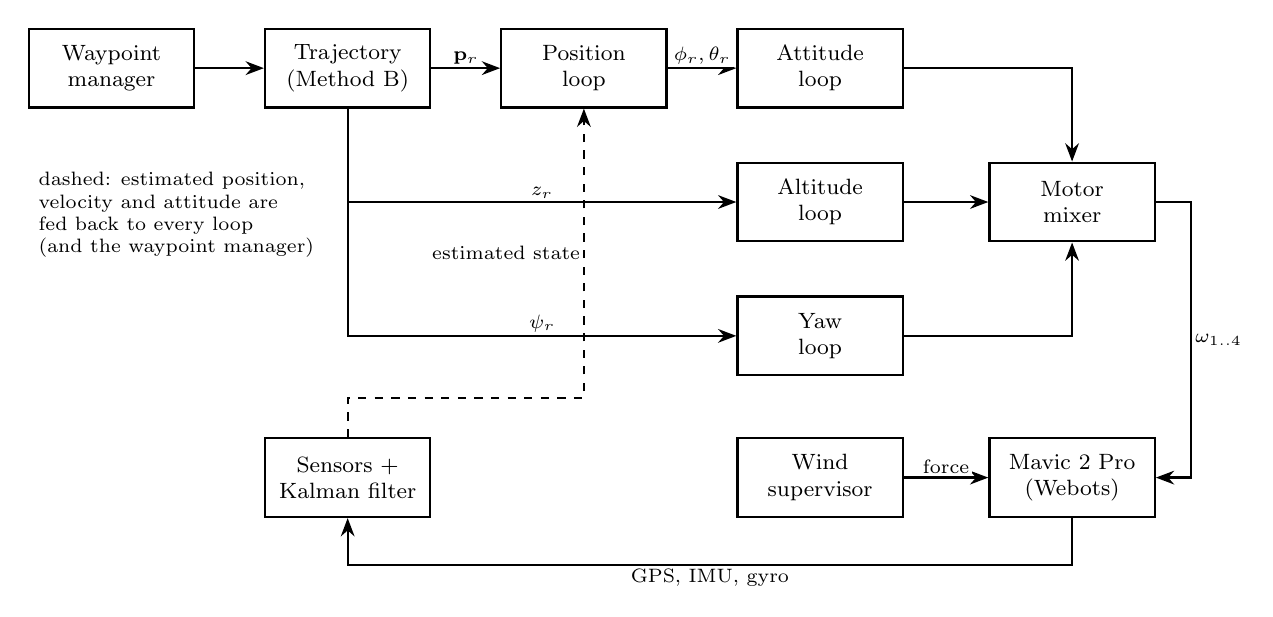
\begin{tikzpicture}[box/.style={draw, thick, minimum width=2.1cm, minimum height=1.0cm, align=center, font=\footnotesize}, lab/.style={font=\scriptsize, fill=white, inner sep=1pt}, >={Stealth}]
% reference chain (top row)
\node[box] (wp)  at (0, 0)    {Waypoint\\manager};
\node[box] (tr)  at (3.0, 0)  {Trajectory\\(Method B)};
\node[box] (pos) at (6.0, 0)  {Position\\loop};
\node[box] (att) at (9.0, 0)  {Attitude\\loop};
% vertical and heading loops (middle)
\node[box] (alt) at (9.0, -1.7) {Altitude\\loop};
\node[box] (yaw) at (9.0, -3.4) {Yaw\\loop};
% actuation and plant (right column)
\node[box] (mix) at (12.2, -1.7) {Motor\\mixer};
\node[box] (dr)  at (12.2, -5.2) {Mavic 2 Pro\\(Webots)};
\node[box] (wnd) at (9.0, -5.2) {Wind\\supervisor};
% estimation (bottom left)
\node[box] (est) at (3.0, -5.2) {Sensors +\\Kalman filter};
\draw[->, thick] (wp) -- (tr);
\draw[->, thick] (tr) -- node[above, lab]{$\mathbf p_r$} (pos);
\draw[->, thick] (pos) -- node[above, lab]{$\phi_r, \theta_r$} (att);
\draw[->, thick] (att.east) -| (mix.north);
\draw[->, thick] (alt) -- (mix);
\draw[->, thick] (yaw.east) -| (mix.south);
\draw[->, thick] (tr.south) |- node[pos=0.75, above, lab]{$z_r$} (alt.west);
\draw[->, thick] (tr.south) |- node[pos=0.75, above, lab]{$\psi_r$} (yaw.west);
\draw[->, thick] (mix.east) -- ++(0.45,0) |- node[pos=0.25, right, lab]{$\omega_{1..4}$} (dr.east);
\draw[->, thick] (wnd) -- node[above, lab]{force} (dr);
\draw[->, thick] (dr.south) -- ++(0,-0.6) -| node[pos=0.25, below, lab]{GPS, IMU, gyro} (est.south);
\draw[->, thick, dashed] (est.north) -- ++(0,0.5) -| node[pos=0.75, left, lab]{estimated state} (pos.south);
\node[font=\scriptsize, align=left, anchor=north west] at (-1.05,-1.2) {dashed: estimated position,\\velocity and attitude are\\fed back to every loop\\(and the waypoint manager)};
\end{tikzpicture}
\caption{System block diagram (the trajectory block is bypassed in Method A)}
\label{fig:block}
\end{figure}

\subsection{Robot and environment}
The robot is the Webots model of the DJI Mavic 2 Pro [4], an X-configuration quadrotor. Its main body has a mass of 0.4\,kg with the centre of mass at $x = -0.088$\,m. The front propellers are at $x = +0.055$\,m and the rear ones at $x = -0.177$\,m, so the rotors are not centred on the centre of mass. The worlds (\texttt{hover.wbt}, \texttt{square.wbt}, \texttt{wind.wbt}) contain a flat 100\,m $\times$ 100\,m floor, the drone starting at $(0, 0, 0.1)$\,m with yaw 0, and a supervisor robot. The physics time step is 8\,ms, and the air damping is 0.5 (linear and angular), as required by the Webots sample controller.

Table~\ref{tab:hw} lists the devices used.

\begin{table}[h]
\centering
\caption{Sensors and actuators of the simulated Mavic 2 Pro}
\label{tab:hw}
\begin{tabular}{|P{3.4cm}|P{3.6cm}|P{5.8cm}|}
\hline
\textbf{Device} & \textbf{Webots name} & \textbf{Use} \\ \hline
GPS & \texttt{gps} & Position $(x, y, z)$; input to the Kalman filter \\ \hline
Inertial unit & \texttt{inertial unit} & Roll, pitch, yaw angles \\ \hline
Gyroscope & \texttt{gyro} & Body rates $p, q, r$ for damping \\ \hline
4 rotational motors & \texttt{front/rear left/right propeller} & Propeller speed, $0$--$576$\,rad/s \\ \hline
\end{tabular}
\end{table}

\subsection{Verified frames and signs}
We did not assume the sign conventions. A probe controller (\texttt{sign\_probe.py}) hovered the drone with the exact law of the Webots sample controller and injected one offset at a time into the roll, pitch and yaw inputs (Figure~\ref{fig:probe}). The measured responses fixed every sign used in the controllers:
\begin{itemize}[itemsep=0pt,topsep=2pt]
\item a positive roll input drives roll negative, and negative roll moves the drone to $+y$;
\item a positive pitch input drives pitch negative, and negative pitch moves the drone to $-x$;
\item a positive yaw input gives a positive (anticlockwise) yaw rate;
\item the gyro rates correlate with the numerical derivatives of the angles with coefficients $+0.99$, $+1.00$ and $+1.00$.
\end{itemize}
The probe also showed that the sample controller, with no position loop, drifts at about 6\,cm/s in $x$ because of the off-centre thrust. A controller with integral action is needed to cancel this bias.

\begin{figure}[h]
\centering
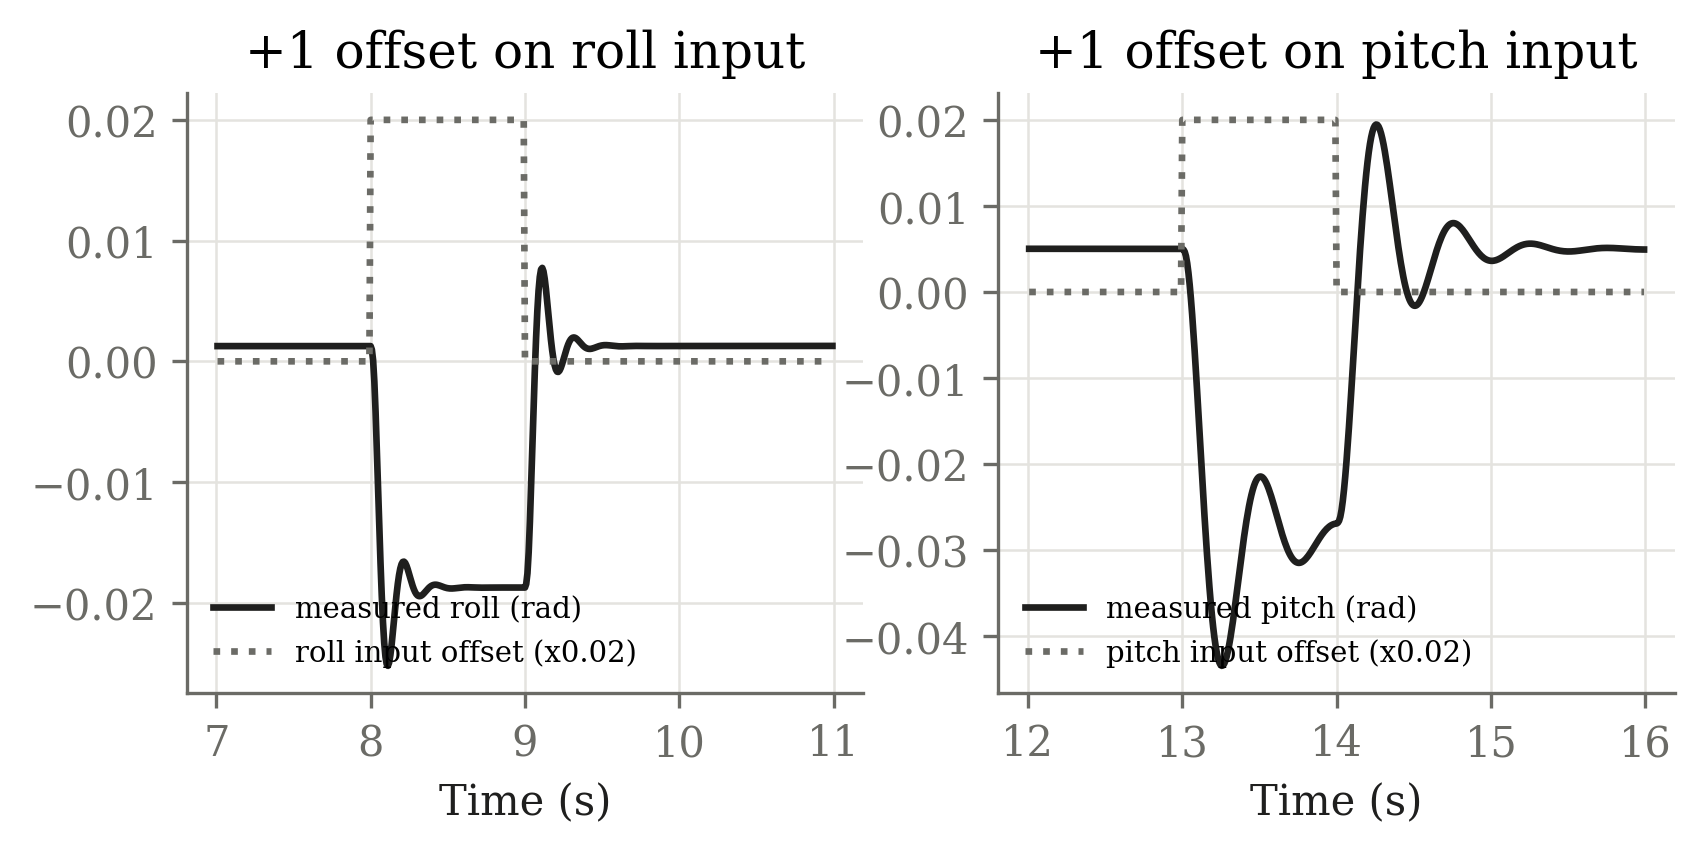
\includegraphics[width=0.92\linewidth]{fig_probe_signs.png}
\caption{Sign probe: response of roll and pitch to a +1 offset on each input}
\label{fig:probe}
\end{figure}

\subsection{Software architecture}
The controller is a Python package with one responsibility per file. Each file has a named owner and its own unit tests (56 tests in total). Table~\ref{tab:files} maps the files to the five team modules.

\begin{table}[h]
\centering
\caption{Software modules and ownership}
\label{tab:files}
\begin{tabular}{|c|P{4.2cm}|P{8cm}|}
\hline
\textbf{Slot} & \textbf{Module} & \textbf{Files} \\ \hline
M1 & State estimation, infrastructure & \texttt{config.py}, \texttt{sensors.py}, \texttt{logger.py}, worlds, sign probe \\ \hline
M2 & Altitude and attitude control & \texttt{pid.py}, \texttt{altitude.py}, \texttt{attitude.py}, \texttt{mixer.py} \\ \hline
M3 & Navigation and trajectory & \texttt{position.py}, \texttt{yaw.py}, \texttt{waypoints.py}, \texttt{trajectory.py} \\ \hline
M4 & Integration and disturbance & \texttt{drone\_main.py}, \texttt{baseline.py}, \texttt{improved.py}, \texttt{wind\_supervisor.py}, \texttt{demo.py} \\ \hline
M5 & Experiments and analysis & \texttt{run\_experiments.py}, \texttt{tune.py}, \texttt{metrics.py}, \texttt{plots.py}, \texttt{tables.py} \\ \hline
\end{tabular}
\end{table}

% Section 7 - written by M4 (Khyati Yadav)
\section{Methodology and Algorithms}
\subsection{Main control loop}
Every 8\,ms the drone controller (1) reads the GPS, inertial unit and gyro, adding Gaussian noise when the scenario asks for it; (2) updates the Kalman filter; (3) calls the selected controller; (4) sends the four rotor speeds; and (5) logs the step. Figure~\ref{fig:flow} shows the flow, including the waypoint switching rule.

\begin{figure}[h]
\centering
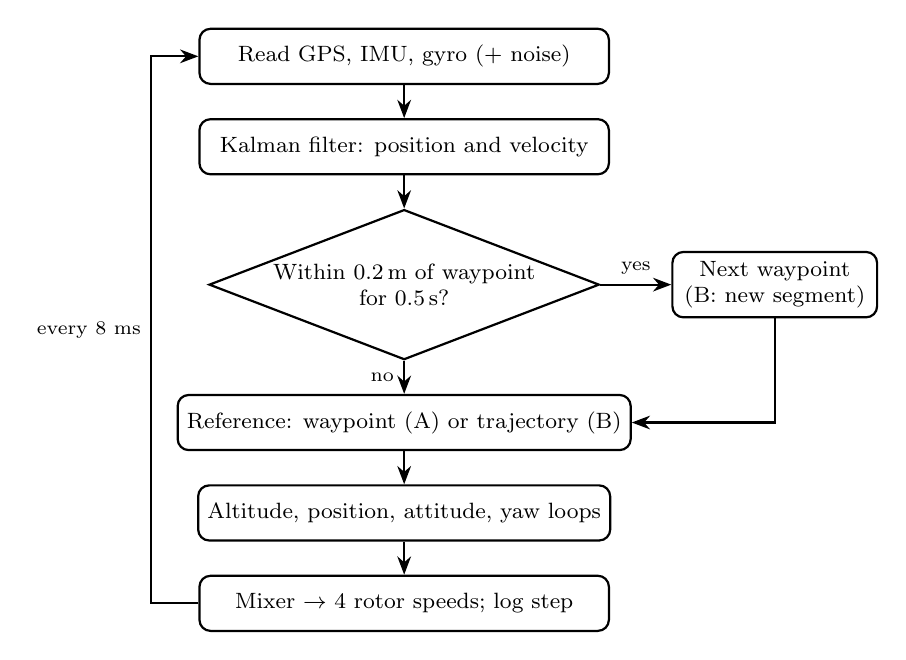
\begin{tikzpicture}[node distance=0.42cm, box/.style={draw, thick, rounded corners, minimum width=5.2cm, minimum height=0.7cm, align=center, font=\footnotesize}, dec/.style={draw, thick, diamond, aspect=2.6, align=center, font=\footnotesize, inner sep=1pt}, >={Stealth}]
\node[box] (a) {Read GPS, IMU, gyro (+ noise)};
\node[box, below=of a] (b) {Kalman filter: position and velocity};
\node[dec, below=of b] (c) {Within 0.2\,m of waypoint\\for 0.5\,s?};
\node[box, below=of c] (d) {Reference: waypoint (A) or trajectory (B)};
\node[box, below=of d] (e) {Altitude, position, attitude, yaw loops};
\node[box, below=of e] (f) {Mixer $\rightarrow$ 4 rotor speeds; log step};
\node[box, right=0.9cm of c, minimum width=2.6cm] (g) {Next waypoint\\(B: new segment)};
\draw[->, thick] (a) -- (b);
\draw[->, thick] (b) -- (c);
\draw[->, thick] (c) -- node[left, font=\scriptsize]{no} (d);
\draw[->, thick] (c) -- node[above, font=\scriptsize]{yes} (g);
\draw[->, thick] (g) |- (d);
\draw[->, thick] (d) -- (e);
\draw[->, thick] (e) -- (f);
\draw[->, thick] (f.west) -- ++(-0.6,0) |- node[left, pos=0.25, font=\scriptsize]{every 8 ms} (a.west);
\end{tikzpicture}
\caption{Flowchart of one control step and the waypoint switching rule}
\label{fig:flow}
\end{figure}

\subsection{Method A: baseline P/PD}
Method A is a faithful, cleaned-up version of the Webots sample. The next waypoint is applied as a step. The altitude loop is PD around the hover speed, the position loop is PD, and the yaw loop is P (Algorithm~\ref{alg:a}). It has no integral term and no feedforward.

\begin{algorithm}[h]
\caption{Method A step (baseline)}
\label{alg:a}
\begin{algorithmic}[1]
\State $w \gets$ current waypoint; advance if reached
\State $u_z \gets K_{pz}(z_w - z) - K_{dz}\,v_z$ \Comment{PD altitude}
\If{$z > 0.3$\,m} \Comment{horizontal loops only once airborne}
\State $\mathbf a \gets K_p(\mathbf p_w - \mathbf p) - K_d\,\mathbf v$ \Comment{PD position, world frame}
\State $(\phi_r, \theta_r) \gets$ tilt from $\mathbf a$ via Eq.~(\ref{eq:rot}), clamped to $\pm 0.15$\,rad
\State $u_\psi \gets K_{p\psi}\,\mathrm{wrap}(\psi_w - \psi)$
\EndIf
\State $u_\phi \gets K_{p\phi}(\phi - \phi_r) + K_{d\phi}\,p$; \quad $u_\theta \gets K_{p\theta}(\theta - \theta_r) + K_{d\theta}\,q$
\State send $\mathrm{mix}(u_z, u_\phi, u_\theta, u_\psi)$ \Comment{Eq.~(\ref{eq:mix})}
\end{algorithmic}
\end{algorithm}

\subsection{Method B: improved trajectory-tracking PID}
Method B keeps the same attitude loop and mixer, so the comparison isolates four changes (Algorithm~\ref{alg:b}):
\begin{enumerate}[itemsep=0pt,topsep=2pt]
\item \textbf{Take-off hand-off.} While on the ground the rotors spool up with a fixed boost. Once the drone is airborne, the first minimum-jerk segment starts from its measured position \emph{and velocity}, so the reference never tells a climbing drone to stop.
\item \textbf{Minimum-jerk reference.} Each waypoint change starts a segment limited to 1.2\,m/s and 1.0\,m/s$^2$. The next waypoint is accepted only once the segment has finished and the drone is within tolerance.
\item \textbf{Altitude PID.} PID with conditional anti-windup, filtered derivative ($\alpha = 0.5$), velocity feedforward, acceleration feedforward (Eq.~\ref{eq:ff}) and tilt compensation.
\item \textbf{Position cascade.} Position P $\rightarrow$ velocity command (limited to 1.5\,m/s) $\rightarrow$ velocity PI with anti-windup $\rightarrow$ acceleration, plus the trajectory's velocity and acceleration as feedforward. The yaw loop is PD.
\end{enumerate}

\begin{algorithm}[h]
\caption{Method B step (improved)}
\label{alg:b}
\begin{algorithmic}[1]
\If{not airborne and no segment planned}
\State send $\mathrm{mix}(u_{boost}, \text{attitude hold}, 0)$; \textbf{return}
\EndIf
\State on first call: plan segment from $(\mathbf p, \psi)$ with start velocity $\mathbf v$
\State advance waypoint only if segment finished and waypoint reached; then plan next segment
\State $(\mathbf p_r, \mathbf v_r, \mathbf a_r) \gets$ trajectory$(t)$
\State $u_z \gets \mathrm{PID}(z_r - z,\; v_{z,r} - v_z) + \omega_h a_{z,r}/(2g)$; \; $u_z \gets (\omega_h + u_z)/\sqrt{\cos\phi\cos\theta} - \omega_h$
\State $\mathbf v_c \gets \mathbf v_r + K_{pp}(\mathbf p_r - \mathbf p)$, $|\mathbf v_c| \le 1.5$
\State $\mathbf a \gets \mathbf a_r + \mathrm{PI}(\mathbf v_c - \mathbf v)$ \Comment{anti-windup}
\State $(\phi_r, \theta_r) \gets$ tilt from $\mathbf a$; $u_\psi \gets K_{p\psi}\mathrm{wrap}(\psi_r - \psi) - K_{d\psi} r$
\State attitude PD and mixer as in Method A
\end{algorithmic}
\end{algorithm}

\subsection{Controller tuning}
Tuning was done in simulation with \texttt{experiments/tune.py}, which runs one scenario with a set of gain overrides and appends the result to a tuning log. Every trial is kept, including those that crashed. The procedure was:
\begin{enumerate}[itemsep=0pt,topsep=2pt]
\item \textbf{Altitude (E1).} Method B's altitude PID gains were raised from $K_p = 4$ to 16 until the step-down overshoot stopped falling. At $K_p = 12$ and above the drone crashed at take-off. This led to two fixes: the velocity-matched take-off hand-off, and the acceleration feedforward, which cut the overshoot from about 8\,\% to 3\,\%. Method A was swept separately. Its best stable setting was $K_p = 12$, $K_d = 8$; at $K_p = 16$ the step command saturated the motors and the drone crashed.
\item \textbf{Attitude (E2 and single-axis tests).} With the sample's roll gain ($K_{p\phi} = 50$) Method A crashed on every square mission. Separate 1\,m moves along $x$ and $y$ isolated the cause to the roll axis. A roll gain of 25 with rate gain 4 is stable, and both methods use it.
\item \textbf{Tilt limit.} With the new roll gains, Method A completed the square up to a tilt limit of 0.15\,rad and crashed at 0.20\,rad. Both methods therefore use 0.15\,rad. Method B flew the square without trouble at peak tilts up to 21$^\circ$ in a separate test with an aggressive (but smooth) trajectory.
\item \textbf{Trajectory speed.} Method B's speed and acceleration limits were swept (speed 1.0--1.5\,m/s with acceleration 0.8--1.2\,m/s$^2$). 1.2\,m/s and 1.0\,m/s$^2$ gave the best trade-off between path error and mission time.
\item \textbf{Estimator (E5).} With the first Kalman setting (process noise $q = 4$\,m$^2$/s$^3$), every noisy run of \emph{both} methods crashed before the first waypoint. The velocity estimate had about 0.26\,m/s of noise, and the altitude derivative gain turned this into thrust jitter, which the off-centre thrust coupled into pitch. Replaying the clean E2 trajectory with added 5\,cm noise offline showed that $q = 0.1$ cuts the velocity error to 0.074\,m/s, while the error without noise changes by only 2\,mm/s. All experiments were then re-run with $q = 0.1$.
\end{enumerate}
Table~\ref{tab:gains} lists the final gains.

\begin{table}[h]
\centering
\caption{Final controller parameters (from \texttt{config.py})}
\label{tab:gains}
\begin{tabular}{|P{5.6cm}|P{3.4cm}|P{3.8cm}|}
\hline
\textbf{Parameter} & \textbf{Method A} & \textbf{Method B} \\ \hline
Altitude $K_p$, $K_i$, $K_d$ & 12, --, 8 & 16, 4, 10 \\ \hline
Roll $K_p$, $K_d$ / pitch $K_p$, $K_d$ & 25, 4 / 30, 2.5 & 25, 4 / 30, 2.5 \\ \hline
Position & PD: $K_p = 1.0$, $K_d = 1.2$ & P 1.2 $\rightarrow$ PI 2.0, 0.5 \\ \hline
Yaw & P: 0.5 & PD: 0.8, 0.3 \\ \hline
Tilt limit / speed limit & 0.15 rad / -- & 0.15 rad / 1.5 m/s \\ \hline
Trajectory limits & -- (steps) & 1.2 m/s, 1.0 m/s$^2$ \\ \hline
\end{tabular}
\end{table}

% Section 8 - written by M4 (Khyati Yadav)
\section{Simulation Setup}
\subsection{Platform}
Webots R2025a [3] with the DJI Mavic 2 Pro model [4]; controllers in Python 3.13 with NumPy, pandas, Matplotlib, PyYAML and pytest; experiments run headless with \texttt{webots --mode=fast --batch --no-rendering}. A supervisor robot (\texttt{wind\_supervisor.py}) applies the wind force with \texttt{addForce}, ends a run early if the drone tilts beyond 60$^\circ$ for one second, and draws the waypoints and a status line in demonstration runs.

\subsection{Experiments}
Table~\ref{tab:scen} defines the six experiments. Both methods run every experiment under identical conditions, from the same YAML file in \texttt{experiments/scenarios/}.

\begin{table}[h]
\centering
\caption{Experiment scenarios}
\label{tab:scen}
\begin{tabular}{|c|P{5.6cm}|P{6.6cm}|}
\hline
\textbf{ID} & \textbf{Scenario} & \textbf{Measures} \\ \hline
E1 & Take-off to 2.0\,m at $t=0$; step to 1.0\,m at $t=15$\,s (timed) & Rise time, overshoot, settling time, steady-state error \\ \hline
E2 & 2\,m $\times$ 2\,m square at 1.5\,m, nose turned along each leg & Path RMSE, max error, mission time, tilt, effort \\ \hline
E3 & Five 3D waypoints, altitude 1.0--2.5\,m & As E2 \\ \hline
E4 & E2 with 0.3\,N crosswind along $+y$ and 0.15\,N gusts (period 4\,s) from $t=8$\,s & Waypoints reached, path error \\ \hline
E5 & E2 with GPS noise $\sigma = 5$\,cm and IMU noise $\sigma = 0.005$\,rad, seeds 1--10 & Success rate, path RMSE mean $\pm$ std \\ \hline
E6 & E2 with roll gain $K_{p\phi} \in \{15, 20, 25, 30, 35, 40, 50\}$ & Success and RMSE vs gain \\ \hline
\end{tabular}
\end{table}

\subsection{Metrics}
All position metrics use the true GPS position, before any injected noise. A run counts as \emph{crashed} if the tilt exceeds 60$^\circ$ or the drone falls below 0.15\,m after having flown above 0.5\,m. It is a \emph{success} if it did not crash and reached every waypoint. Path RMSE is the root-mean-square distance from the drone to the straight-line path through the waypoints, from the first waypoint until the mission ends. Control effort is the time-average of $\sum_i(\omega_i - \omega_h)^2$. Step metrics follow the usual definitions [11], with a $\pm2\,\%$ settling band.

\subsection{How to run}
\begin{verbatim}
pip install -r requirements.txt
make test                              # 56 unit tests
python experiments/run_experiments.py   # all runs
python analysis/plots.py               # figures
python analysis/tables.py              # tables, numbers
make report                            # this PDF
python experiments/demo.py E2 improved # live demo
python experiments/demo.py --points "0,0,1.5 2,1,2 0,0,1" baseline
\end{verbatim}

% Section 9 - written by M5 (Ambrish Chauraiya). All numbers come from results/summary.csv
% through report/generated/*.tex (analysis/tables.py); none are typed by hand.
\section{Results and Analysis}
Both methods ran every experiment in Table~\ref{tab:scen}, 42 runs in total. Tables~\ref{tab:e1}--\ref{tab:e6} and Figures~\ref{fig:e1}--\ref{fig:e6} are generated directly from the logged telemetry.

\subsection{E1: altitude step response}
Figure~\ref{fig:e1} and Table~\ref{tab:e1} show the altitude response. Method A has no integral term, so it settles \R{E1}{baseline}{step2_ss_error_m}\,m below the target in both steps. The hover speed it assumes (68.5\,rad/s, taken from the sample) is slightly lower than the true hover speed, and nothing corrects for that. Because of this offset it never enters the $\pm2\,\%$ band, so its settling time is undefined. Method B's integral term removes the offset: its steady-state error is \R{E1}{improved}{step2_ss_error_m}\,m. On the 2\,m $\to$ 1\,m step its overshoot is \R{E1}{improved}{step2_overshoot_pct}\,\%, against \R{E1}{baseline}{step2_overshoot_pct}\,\% for Method A. Method B rises more slowly (\R{E1}{improved}{step1_rise_time_s}\,s against \R{E1}{baseline}{step1_rise_time_s}\,s at take-off). This is deliberate: it follows a smooth reference rather than the raw step.

\begin{figure}[H]
\centering
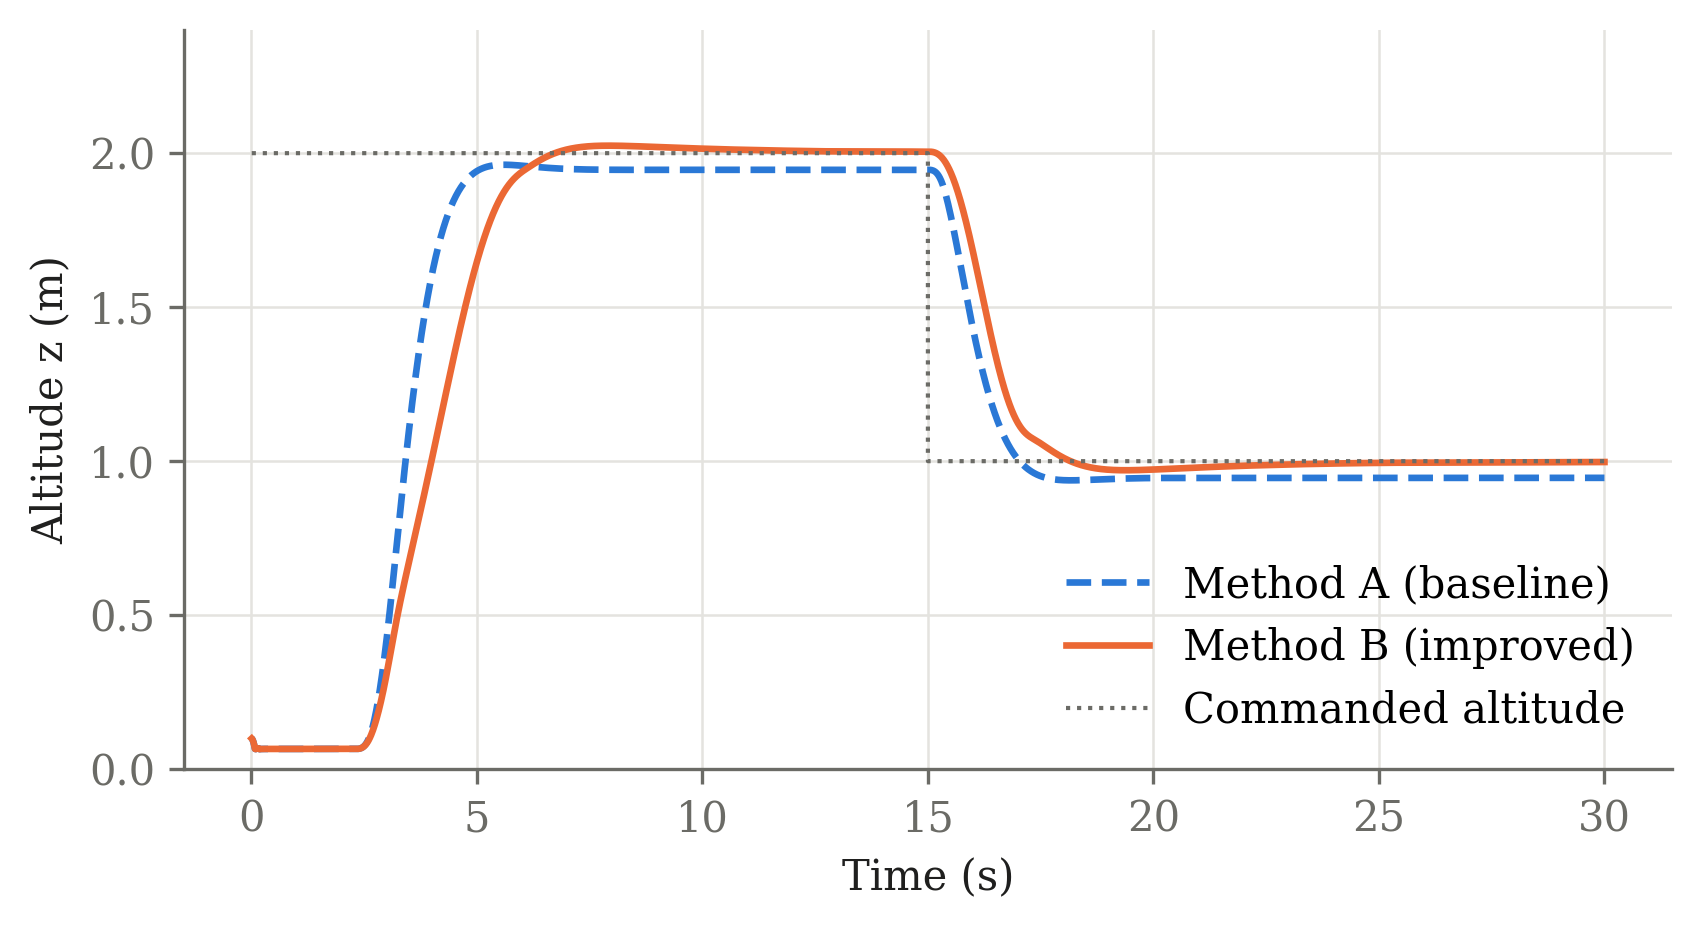
\includegraphics[width=0.62\linewidth]{fig_e1_step_response.png}
\caption{E1 altitude step response (true altitude)}
\label{fig:e1}
\end{figure}

\begin{table}[h]
\centering
\caption{E1 altitude step response (true altitude)}
\label{tab:e1}
\begin{tabular}{|p{8.2cm}|c|c|}
\hline
\textbf{Metric} & \textbf{Method A} & \textbf{Method B} \\ \hline
Take-off 0.1 m $\to$ 2.0 m: Rise time 10--90\% (s) & 1.50 & 2.41 \\ \hline
Take-off 0.1 m $\to$ 2.0 m: Overshoot (\%) & 0.0 & 1.3 \\ \hline
Take-off 0.1 m $\to$ 2.0 m: Settling time, 2\% band (s) & -- & 6.2 \\ \hline
Take-off 0.1 m $\to$ 2.0 m: Steady-state error (m) & 0.054 & 0.005 \\ \hline
Step 2.0 m $\to$ 1.0 m: Rise time 10--90\% (s) & 1.30 & 1.50 \\ \hline
Step 2.0 m $\to$ 1.0 m: Overshoot (\%) & 6.2 & 2.9 \\ \hline
Step 2.0 m $\to$ 1.0 m: Settling time, 2\% band (s) & -- & 6.1 \\ \hline
Step 2.0 m $\to$ 1.0 m: Steady-state error (m) & 0.054 & 0.003 \\ \hline
\end{tabular}
\end{table}


\subsection{E2 and E3: waypoint missions}
On the square mission (Figure~\ref{fig:e2}) both methods reach all five waypoints. Method A's path RMSE is \R{E2}{baseline}{path_rmse_m}\,m and Method B's \R{E2}{improved}{path_rmse_m}\,m (Table~\ref{tab:e2e3}). The larger differences are in how the drone is driven. Method A sees every new waypoint as a 2\,m step and immediately commands the full tilt limit. Figure~\ref{fig:tilt} shows its tilt spikes at each corner, peaking at \R{E2}{baseline}{max_tilt_deg}$^\circ$ against \R{E2}{improved}{max_tilt_deg}$^\circ$. Method B's control effort is \R{E2}{reduction}{control_effort}\,\% lower, and it finishes the mission sooner (\R{E2}{improved}{mission_time_s}\,s against \R{E2}{baseline}{mission_time_s}\,s). On the 3D mission (Figure~\ref{fig:e3}) the gap is larger. Method A's altitude offset and step commands give a path RMSE of \R{E3}{baseline}{path_rmse_m}\,m, against \R{E3}{improved}{path_rmse_m}\,m for Method B, an \R{E3}{reduction}{path_rmse_m}\,\% reduction.

\begin{figure}[H]
\centering
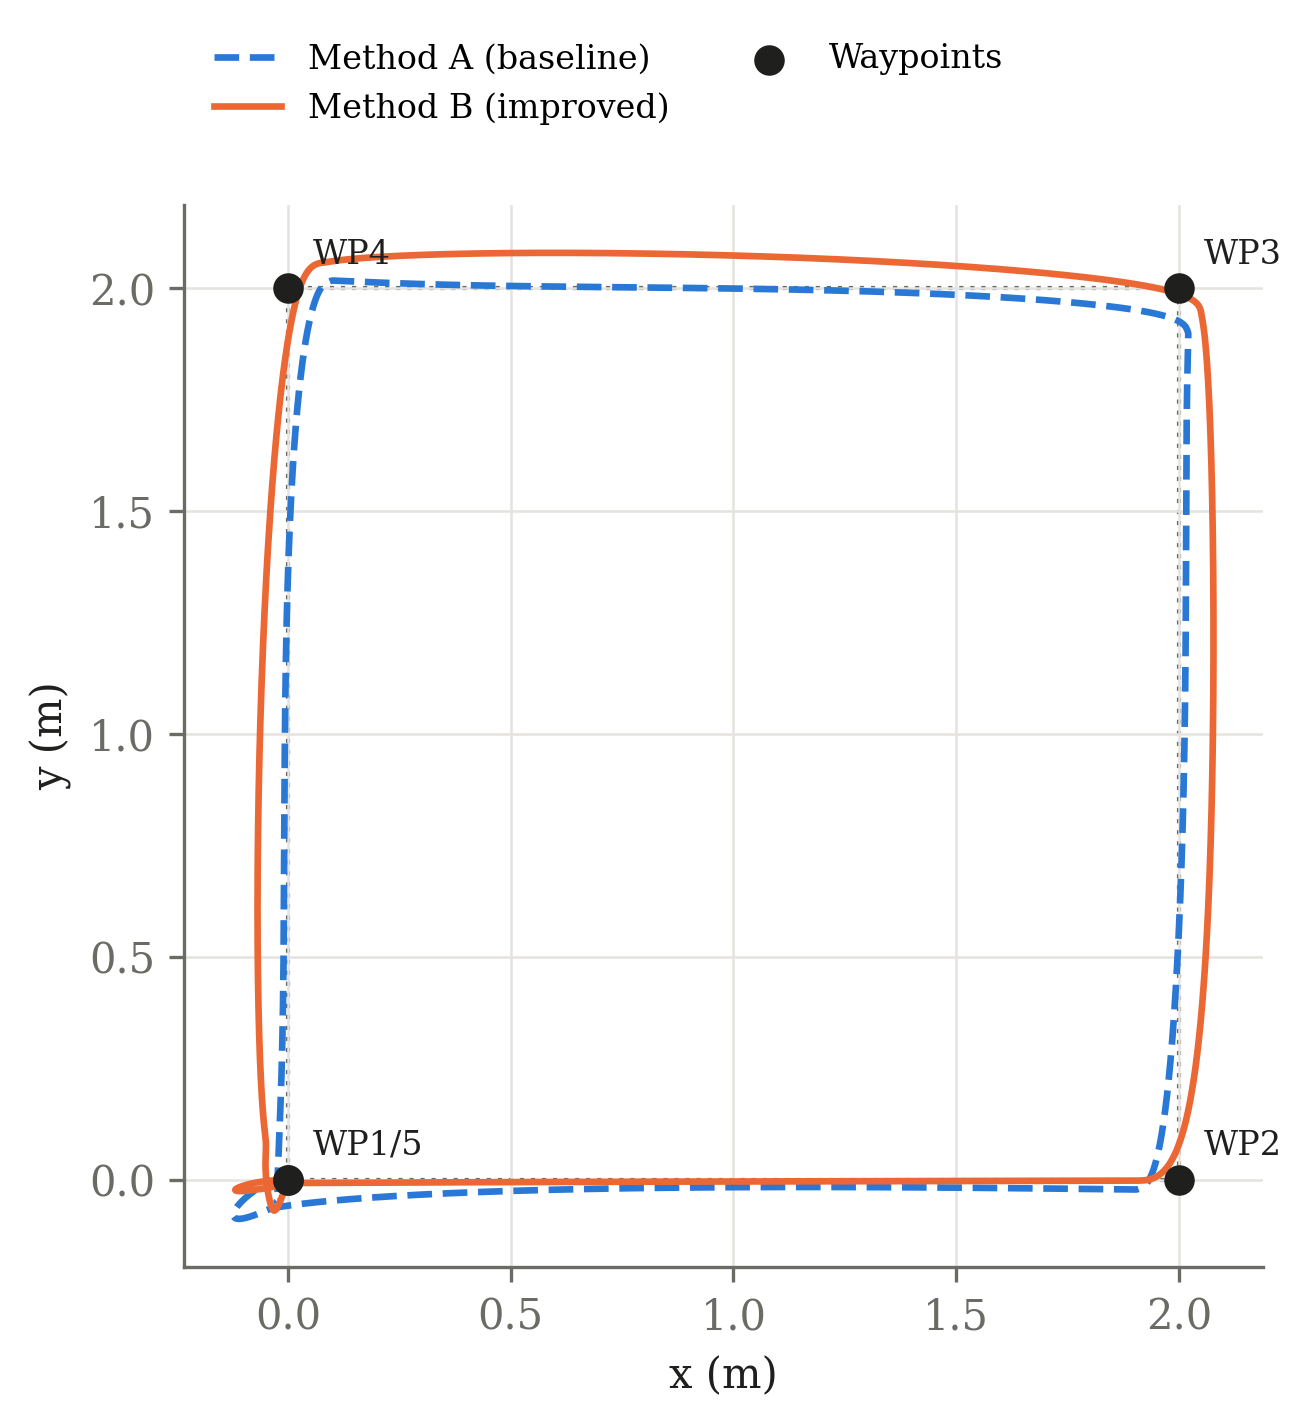
\includegraphics[width=0.45\linewidth]{fig_e2_xy_path.png}
\caption{E2 square mission, top view}
\label{fig:e2}
\end{figure}

\begin{figure}[H]
\centering
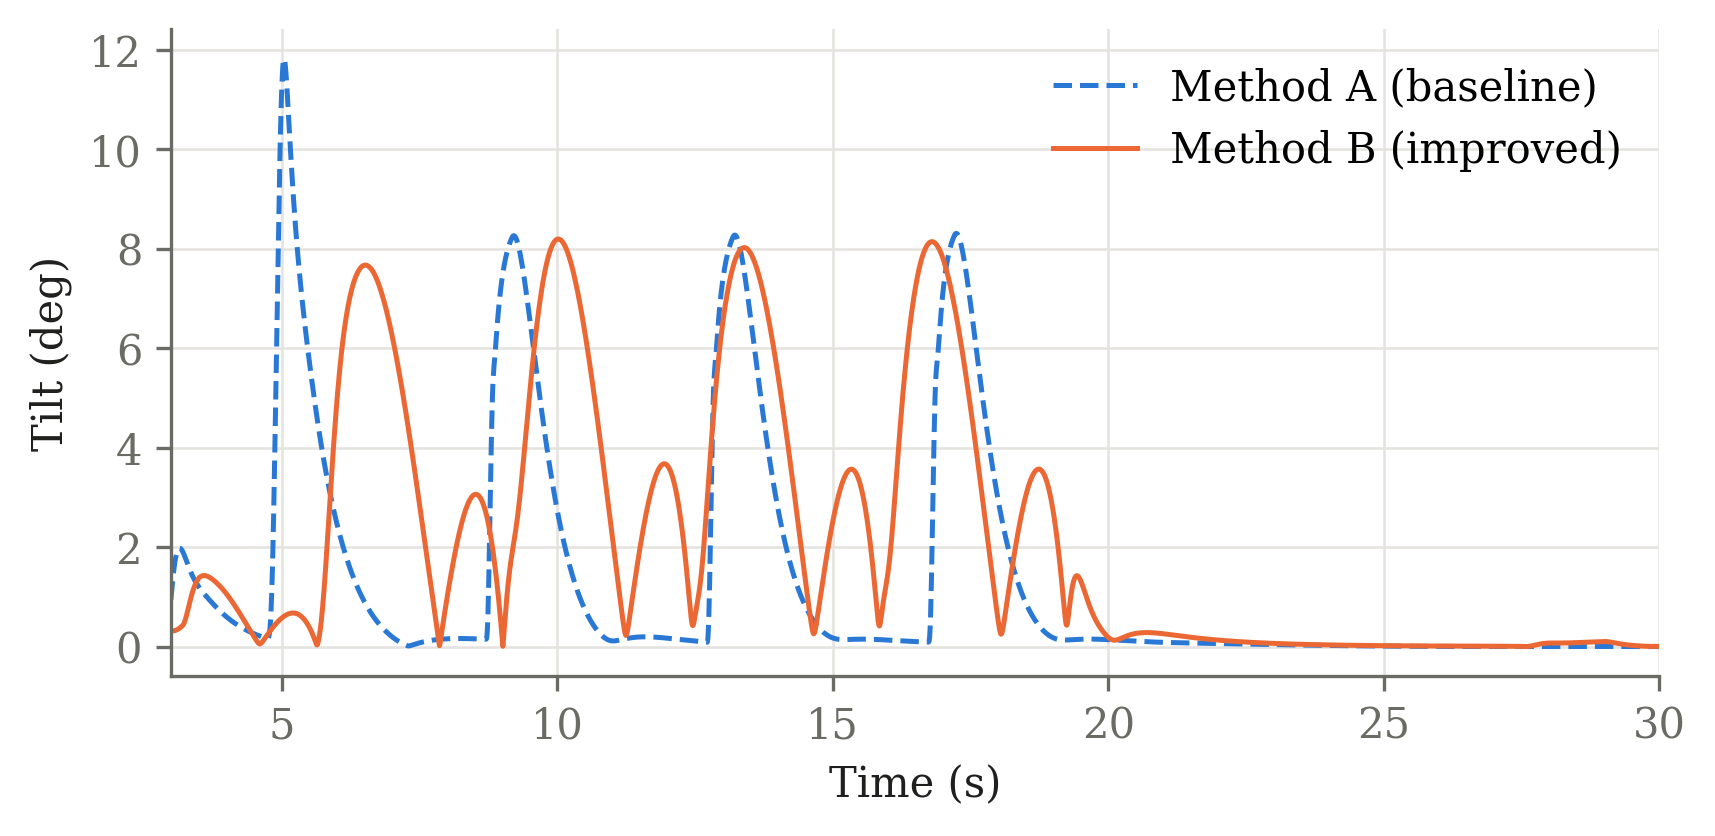
\includegraphics[width=0.62\linewidth]{fig_e2_tilt.png}
\caption{E2 tilt angle over time: step commands cause tilt spikes at each corner}
\label{fig:tilt}
\end{figure}

\begin{figure}[H]
\centering
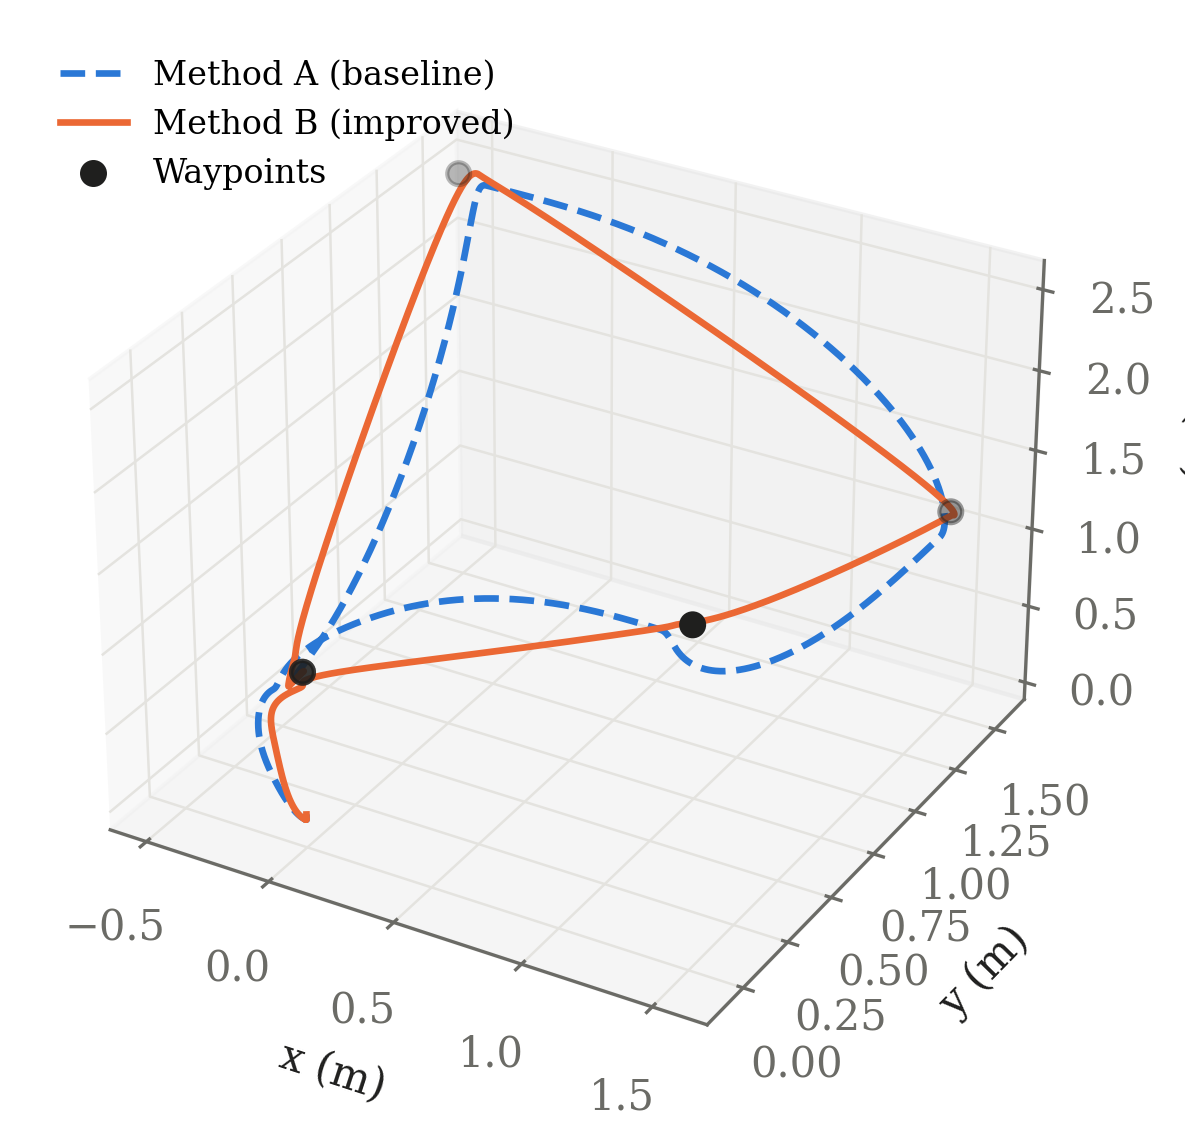
\includegraphics[width=0.44\linewidth]{fig_e3_3d_path.png}
\caption{E3 3D waypoint mission}
\label{fig:e3}
\end{figure}

\begin{table}[h]
\centering
\caption{Waypoint missions without disturbance (E2, E3)}
\label{tab:e2e3}
\begin{tabular}{|p{8.2cm}|c|c|}
\hline
\textbf{Metric} & \textbf{Method A} & \textbf{Method B} \\ \hline
E2 square: Path RMSE (m) & 0.063 & 0.049 \\ \hline
E2 square: Max path error (m) & 0.109 & 0.080 \\ \hline
E2 square: Mission time (s) & 20.8 & 19.2 \\ \hline
E2 square: Peak tilt (deg) & 11.8 & 8.2 \\ \hline
E2 square: Control effort ((rad/s)$^2$) & 27.1 & 12.1 \\ \hline
E3 3D: Path RMSE (m) & 0.275 & 0.046 \\ \hline
E3 3D: Max path error (m) & 0.542 & 0.068 \\ \hline
E3 3D: Mission time (s) & 20.4 & 18.7 \\ \hline
E3 3D: Peak tilt (deg) & 10.2 & 7.4 \\ \hline
E3 3D: Control effort ((rad/s)$^2$) & 35.2 & 12.6 \\ \hline
\end{tabular}
\end{table}


\subsection{E4: crosswind}
From $t = 8$\,s a 0.3\,N crosswind with 0.15\,N gusts pushes the drone along $+y$ (Figures~\ref{fig:e4path} and \ref{fig:e4}). Method A has no integral action. Its position loop needs a steady error to produce the force that balances the wind, so the drone settles about 0.5\,m downwind of the path. That is outside the 0.2\,m arrival tolerance, so Method A reaches only \R{E4}{baseline}{waypoints_reached} of 5 waypoints and never finishes. It does not crash. Method B's velocity-loop integral builds up a constant tilt into the wind. It reaches all five waypoints in \R{E4}{improved}{mission_time_s}\,s with a path RMSE of \R{E4}{improved}{path_rmse_m}\,m (Table~\ref{tab:e4}). The gusts remain visible in Figure~\ref{fig:e4} as small periodic errors, because the integral can cancel the mean force but not the 4\,s oscillation.

\begin{figure}[H]
\centering
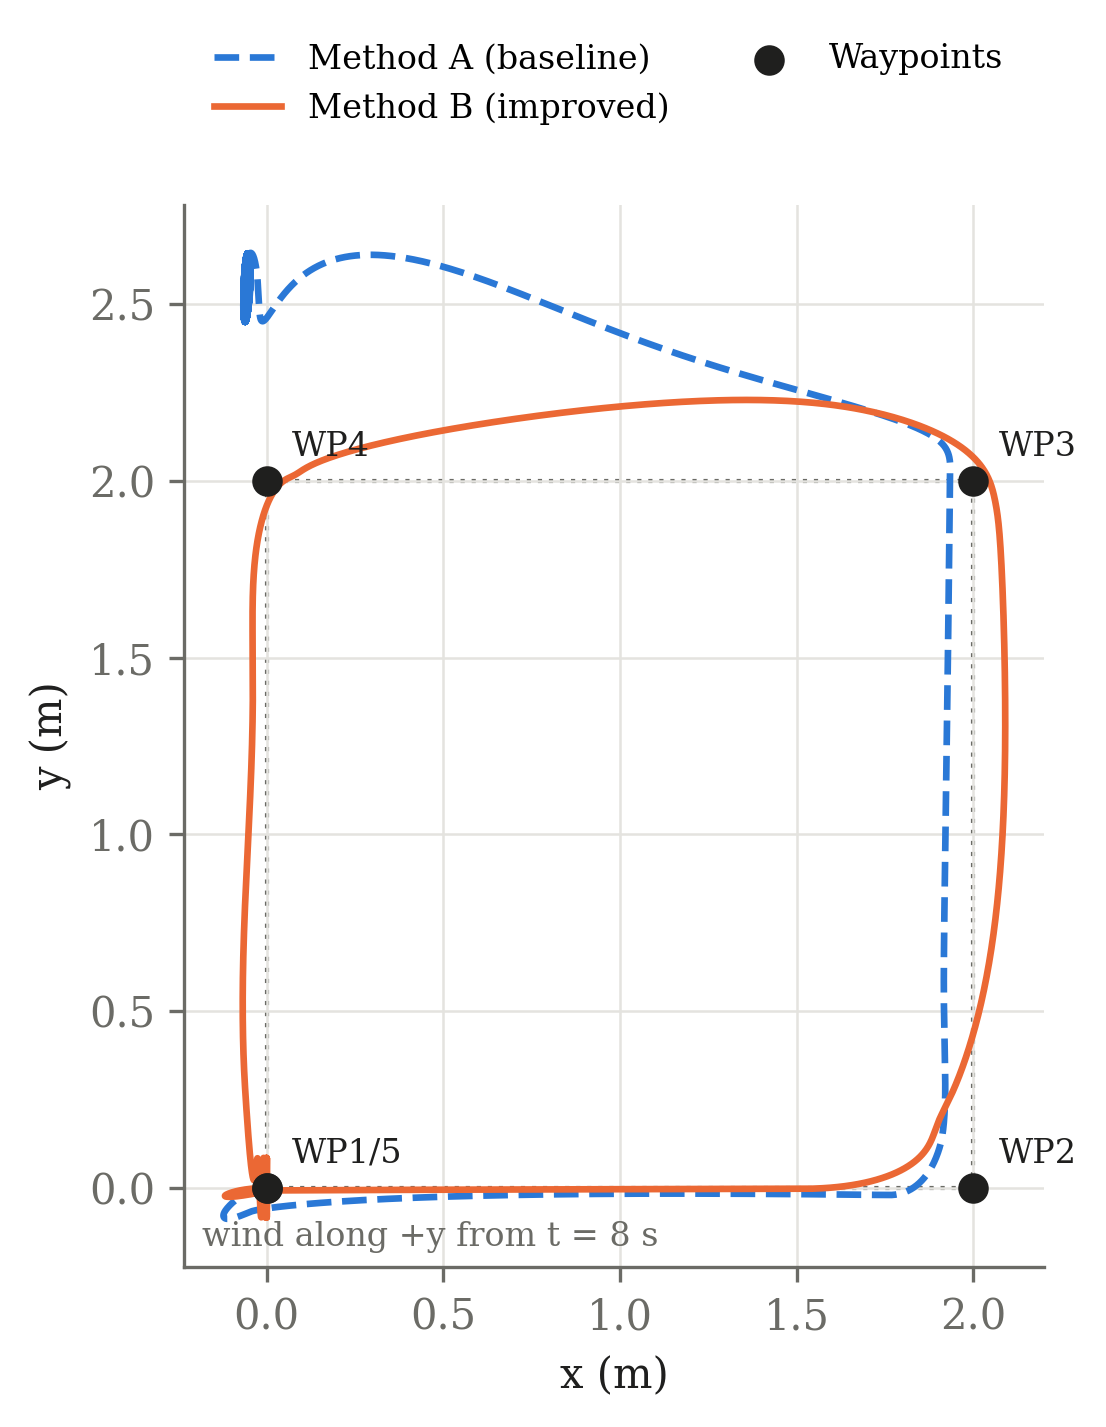
\includegraphics[width=0.45\linewidth]{fig_e4_xy_path.png}
\caption{E4 square mission under crosswind, top view}
\label{fig:e4path}
\end{figure}

\begin{figure}[H]
\centering
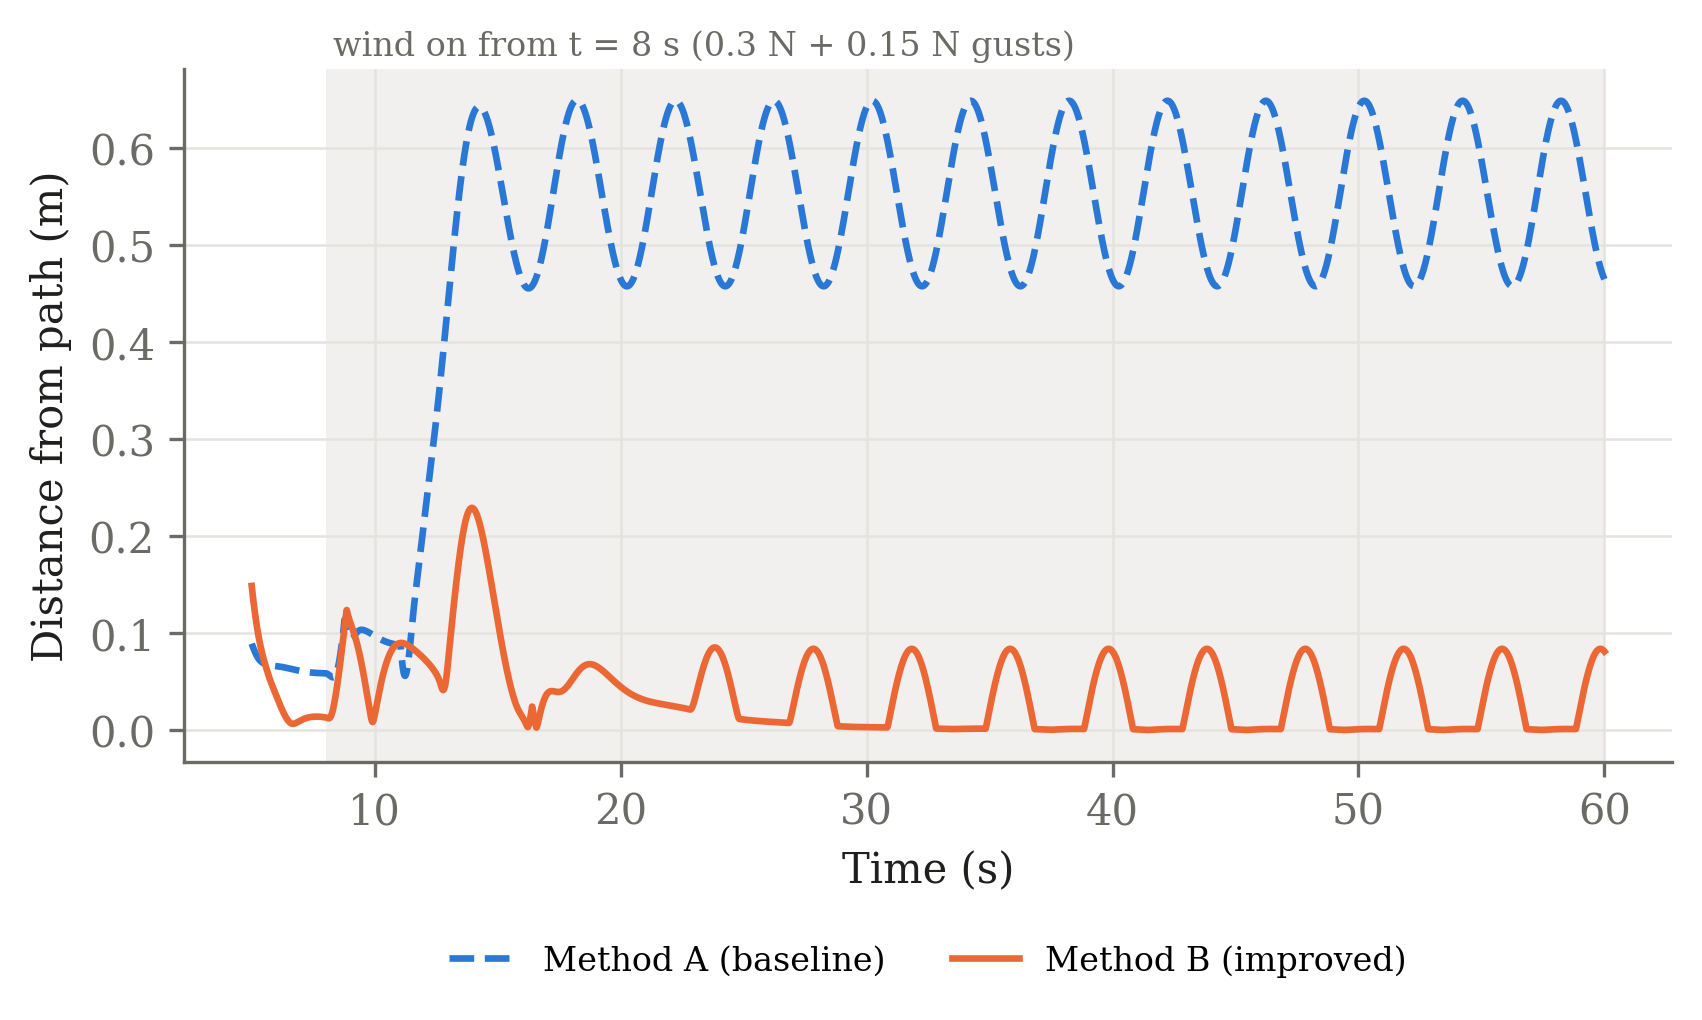
\includegraphics[width=0.62\linewidth]{fig_e4_wind_error.png}
\caption{E4 distance from the planned path over time}
\label{fig:e4}
\end{figure}

\begin{table}[h]
\centering
\caption{Square mission under crosswind (E4)}
\label{tab:e4}
\begin{tabular}{|p{8.2cm}|c|c|}
\hline
\textbf{E4 metric (wind 0.3 N + 0.15 N gusts)} & \textbf{Method A} & \textbf{Method B} \\ \hline
Waypoints reached (of 5) & 3 & 5 \\ \hline
Path RMSE (m) & 0.517 & 0.086 \\ \hline
Max path error (m) & 0.650 & 0.229 \\ \hline
Mission time (s) & -- & 20.0 \\ \hline
Peak tilt (deg) & 13.4 & 11.1 \\ \hline
\end{tabular}
\end{table}


\subsection{E5: sensor noise}
With 5\,cm GPS noise and 0.005\,rad IMU noise, each method flew the square ten times with different random seeds (Table~\ref{tab:e5}, Figure~\ref{fig:e5}). Method B succeeded in \R{E5}{improved}{success} runs, and its path RMSE was almost unchanged from the noise-free case (\R{E5}{improved}{mean_path_rmse_m}\,$\pm$\,\R{E5}{improved}{std_path_rmse_m}\,m against \R{E2}{improved}{path_rmse_m}\,m in E2). Method A succeeded in \R{E5}{baseline}{success} runs and crashed in \R{E5}{baseline}{crash_count}. Its step commands drive the attitude loop hard (Section 9.5), which probably left too little margin for the extra noise in those seeds; we did not log the signals needed to confirm this. This experiment also exposed a real weakness of our first design. With the initial Kalman filter setting every noisy run of both methods crashed, and the estimator had to be retuned (Section 7.4). The noise result therefore depends as much on the shared estimator as on the controller.

\begin{figure}[H]
\centering
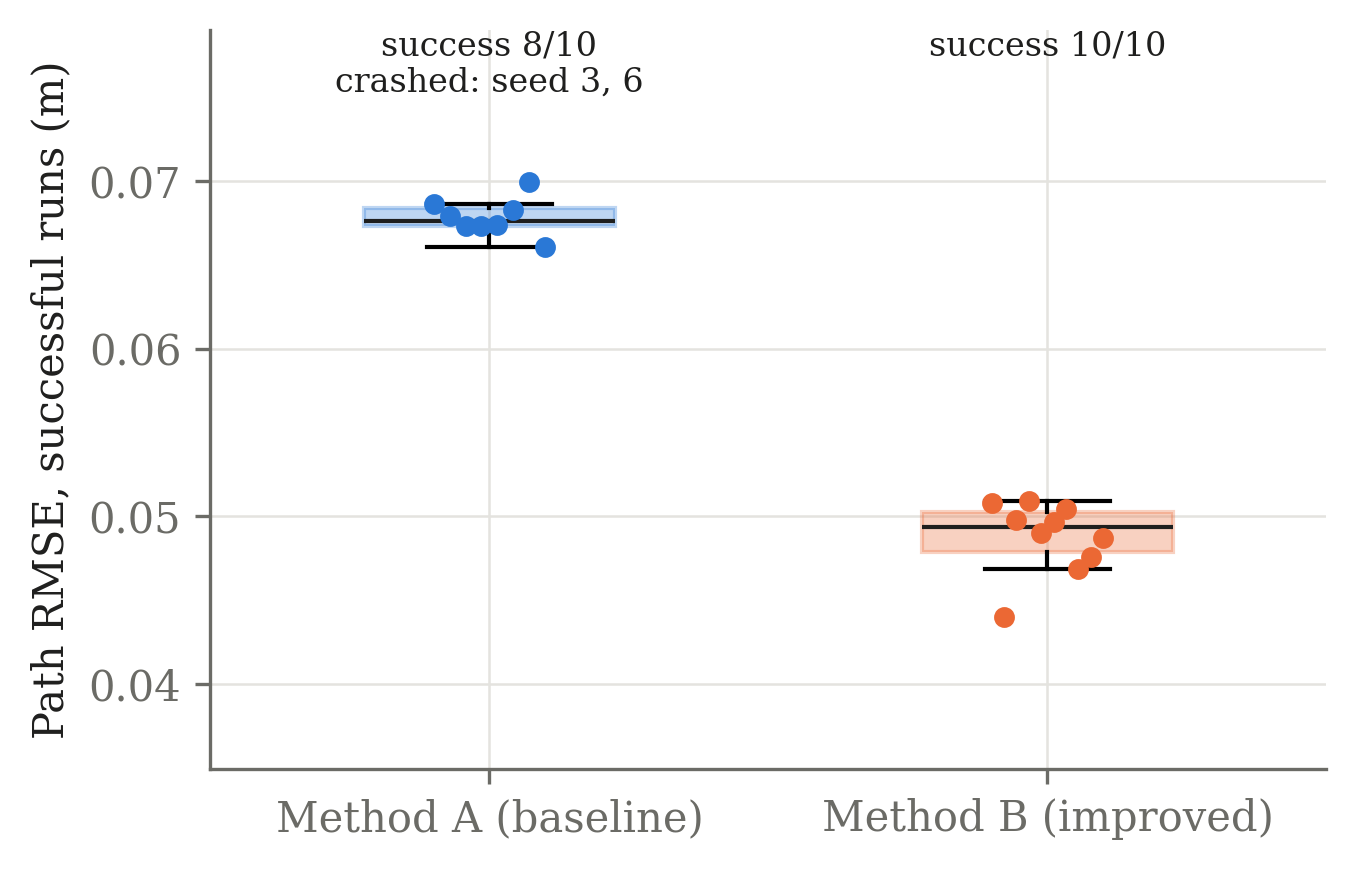
\includegraphics[width=0.48\linewidth]{fig_e5_noise_box.png}
\caption{E5 path RMSE over ten noise seeds}
\label{fig:e5}
\end{figure}

\begin{table}[h]
\centering
\caption{Sensor-noise robustness over ten seeds (E5, mean $\pm$ std of successful runs)}
\label{tab:e5}
\begin{tabular}{|l|c|c|c|c|}
\hline
\textbf{Method} & \textbf{Success} & \textbf{Path RMSE (m)} & \textbf{Mission time (s)} & \textbf{Peak tilt (deg)} \\ \hline
Method A & 8/10 & 0.068 $\pm$ 0.001 & 21.4 $\pm$ 0.3 & 12.6 \\ \hline
Method B & 10/10 & 0.049 $\pm$ 0.002 & 19.5 $\pm$ 0.2 & 9.8 \\ \hline
\end{tabular}
\end{table}


\subsection{E6: roll-gain sensitivity}
The roll proportional gain was swept from 15 to 50, the value used in the Webots sample (Table~\ref{tab:e6}, Figure~\ref{fig:e6}). Method A crashed at $K_{p\phi} \in \{$\R{E6}{baseline}{failed_gains}$\}$, including the sample's own value. Method B completed the mission at every gain (no failures). Both methods use the same attitude loop, so the difference comes from the commands it receives. In the single-axis tests the drone flipped at large roll gains. Our interpretation is that step waypoints demand a sudden large tilt, which a stiff roll loop answers with growing oscillation, while the smooth reference keeps the attitude loop in its small-signal range; we did not log the internal signals that would prove this. Method B is thus much less sensitive to how the inner loop is tuned.

\begin{figure}[H]
\centering
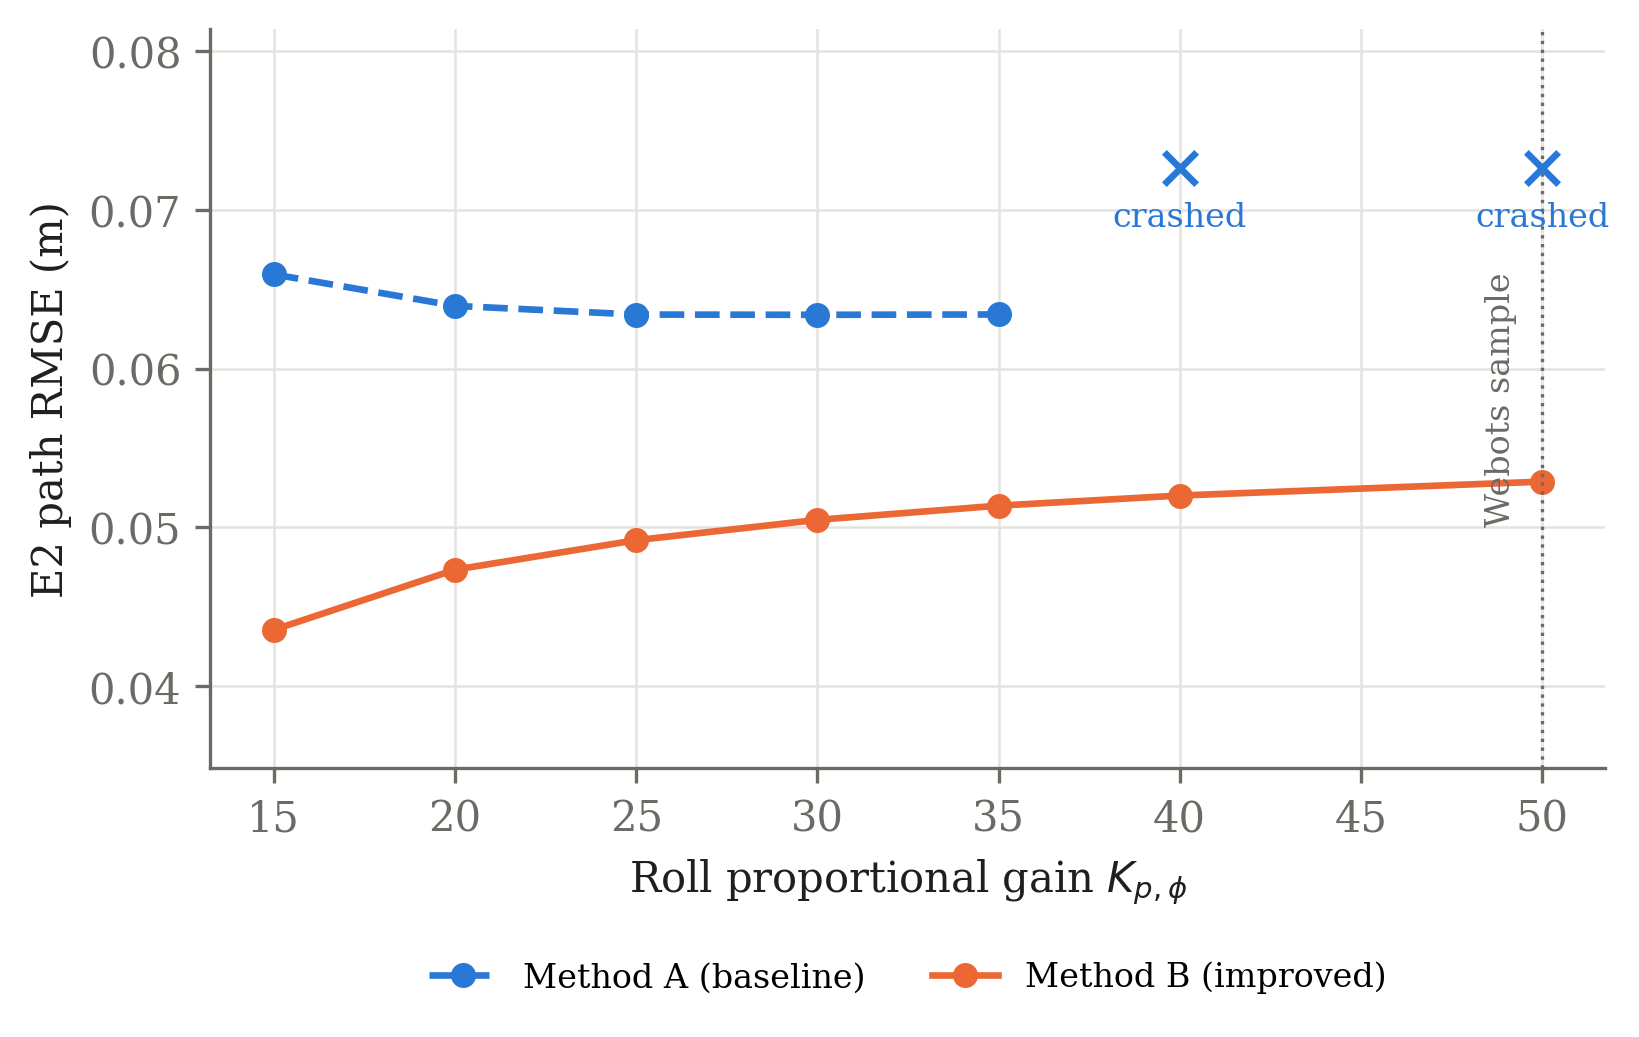
\includegraphics[width=0.65\linewidth]{fig_e6_roll_gain_sweep.png}
\caption{E6 roll-gain sweep: path RMSE of successful runs; crosses mark failed runs}
\label{fig:e6}
\end{figure}

\begin{table}[h]
\centering
\caption{Roll-gain sensitivity on the square mission (E6)}
\label{tab:e6}
\begin{tabular}{|c|c|c|}
\hline
\textbf{Roll $K_p$} & \textbf{Method A} & \textbf{Method B} \\ \hline
15 & success, RMSE 0.066 m & success, RMSE 0.044 m \\ \hline
20 & success, RMSE 0.064 m & success, RMSE 0.047 m \\ \hline
25 & success, RMSE 0.063 m & success, RMSE 0.049 m \\ \hline
30 & success, RMSE 0.063 m & success, RMSE 0.050 m \\ \hline
35 & success, RMSE 0.063 m & success, RMSE 0.051 m \\ \hline
40 & crashed & success, RMSE 0.052 m \\ \hline
50 & crashed & success, RMSE 0.053 m \\ \hline
\end{tabular}
\end{table}


\subsection{What worked and what did not}
\begin{itemize}[itemsep=0pt,topsep=2pt]
\item \textbf{Worked:} measuring the sign conventions first. The pre-project controller had the attitude sign inverted and flipped on every run. Integral action removed the altitude offset and the wind offset. The smooth reference reduced tilt and control effort and made the system tolerant of the roll gain.
\item \textbf{Did not work at first:} the sample's roll gain of 50 was unstable for larger tilt; Method B's first take-off crashed because the reference ignored the climb speed; and the first estimator setting failed under noise. Each failure is recorded in the tuning log, and each fix is described in Section 7.
\item \textbf{Limits:} the simulator has no motor delay, battery sag or ground effect; wind is a force, not airflow; and results are for one drone model and missions of a few metres. Method B also rises more slowly than Method A, because of its smooth reference.
\end{itemize}

% Section 10 - every member writes and signs their own row
\section{Contribution}
Table~\ref{tab:contrib} lists the technical contribution of each member. Every item can be traced to the member's commits in the GitHub repository (Appendix) and to their part of the demonstration video.

\renewcommand{\arraystretch}{1.4}
\begin{longtable}{|c|P{2.9cm}|P{6.9cm}|P{2.5cm}|}
\caption{Technical contribution of each member}\label{tab:contrib}\\
\hline
\textbf{S. No.} & \textbf{Name and SAP ID} & \textbf{Technical contribution (modules / algorithms / code files / experiments)} & \textbf{Sections + signature} \\ \hline
\endfirsthead
\hline
\textbf{S. No.} & \textbf{Name and SAP ID} & \textbf{Technical contribution} & \textbf{Sections + signature} \\ \hline
\endhead
1 & Saksham Agrawal (500121969) & State estimation and infrastructure (M1): sign-convention probe in Webots (\texttt{sign\_probe.py}, \texttt{probe.wbt}, \texttt{analyse\_probe.py}) and the verified frames document (\texttt{docs/frames.md}, Fig.~\ref{fig:probe}); constant-velocity Kalman velocity estimator and noise injection (\texttt{sensors.py}); scenario/gain configuration (\texttt{config.py}); telemetry logger (\texttt{logger.py}); the three worlds; repository setup; verified reference list. & Abstract, 1, 2, 13 \\ \hline
2 & Khushi Gupta (500119129) & Altitude and attitude control (M2): PID with conditional anti-windup and filtered derivative (\texttt{pid.py}); Method A PD and Method B PID altitude loops with acceleration feedforward and tilt compensation (\texttt{altitude.py}); attitude PD with the verified sign (\texttt{attitude.py}); motor mixer (\texttt{mixer.py}); altitude and roll-gain tuning (E1, E6); unit tests for these files. & 3, 4 \\ \hline
3 & Tanvi Singhal (500126859) & Navigation and trajectory (M3): Method A PD and Method B position-velocity cascade with body-frame rotation (\texttt{position.py}); yaw controller with angle wrapping (\texttt{yaw.py}); waypoint state machine with timed mode (\texttt{waypoints.py}); quintic minimum-jerk trajectory with non-zero start velocity (\texttt{trajectory.py}); unit tests for these files. & 5, 6 \\ \hline
4 & Khyati Yadav (500123608) & Integration and disturbance (M4): Method A and Method B assemblies including the take-off hand-off (\texttt{baseline.py}, \texttt{improved.py}); controller entry point (\texttt{drone\_main.py}); wind/gust supervisor with crash watchdog, waypoint markers and status labels (\texttt{wind\_supervisor.py}); live demo launcher with custom target points (\texttt{demo.py}); E4 wind experiment. & 7, 8 \\ \hline
5 & Ambrish Chauraiya (500120274) & Experiments and analysis (M5): batch runner and E1--E6 scenario files (\texttt{run\_experiments.py}); tuning harness and tuning log (\texttt{tune.py}); crash-aware metrics (\texttt{metrics.py}); all result figures and tables (\texttt{plots.py}, \texttt{tables.py}, Figs.~\ref{fig:e1}--\ref{fig:e6}, Tables~\ref{tab:e1}--\ref{tab:e6}); E5 Monte Carlo study. & 9, 12, Appendix \\ \hline
\end{longtable}
\renewcommand{\arraystretch}{1.2}

% Section 11 - EACH MEMBER writes their own 5-8 lines in their own words.
% Replace each prompt below with your reflection. Do not let anyone else write it for you.
\section{Co-learning Reflection}
Each member answers three questions in 5--8 lines: what I learned on my own, what I learned from team-mates, and what I taught others.

\textbf{Saksham Agrawal (M1):} \note{To be written by Saksham: e.g. learning the Webots API and frames on your own; what you learned from the control/trajectory members; what you explained to others (for example the sign probe and the Kalman filter).}

\textbf{Khushi Gupta (M2):} \note{To be written by Khushi: e.g. PID tuning and anti-windup; what you learned about frames or trajectories from others; what you taught about the attitude loop and the roll-gain finding.}

\textbf{Tanvi Singhal (M3):} \note{To be written by Tanvi: e.g. trajectory polynomials and body-frame rotation; what you learned from others; what you taught about the minimum-jerk reference.}

\textbf{Khyati Yadav (M4):} \note{To be written by Khyati: e.g. integrating the modules and the Webots supervisor; what you learned from others; what you taught about running the demo and the wind test.}

\textbf{Ambrish Chauraiya (M5):} \note{To be written by Ambrish: e.g. designing fair experiments and metrics; what you learned from others; what you taught about reading the result plots.}

% Section 12 - written by M5 (Ambrish Chauraiya)
\section{Conclusion and Future Scope}
\subsection{Main findings}
We built and compared two complete altitude and waypoint controllers for the Webots DJI Mavic 2 Pro, on top of sign conventions we measured ourselves.
\begin{itemize}[itemsep=0pt,topsep=2pt]
\item Integral action removed the steady altitude error (\R{E1}{baseline}{step2_ss_error_m}\,m $\to$ \R{E1}{improved}{step2_ss_error_m}\,m) and let the drone finish its mission in a crosswind, where the baseline stalled.
\item A minimum-jerk reference reduced peak tilt and cut control effort by \R{E2}{reduction}{control_effort}\,\% on the square mission, without making the mission slower.
\item The smooth reference made the system tolerant of the inner-loop gain. The baseline crashed at roll gains \R{E6}{baseline}{failed_gains}; the improved controller never did.
\item Under GPS and IMU noise, performance depended strongly on the shared Kalman estimator. After retuning it, Method A succeeded in \R{E5}{baseline}{success} runs and Method B in \R{E5}{improved}{success}.
\end{itemize}
Against the objectives of Section 2: the sign model was verified; Method B met the altitude targets (overshoot \R{E1}{improved}{step2_overshoot_pct}\,\%, steady-state error \R{E1}{improved}{step2_ss_error_m}\,m) while Method A missed the steady-state target; both methods met the 0.10\,m path target on the square, but only Method B met it on the 3D mission; and only Method B completed the wind mission.

\subsection{Industrial use}
The improved structure is the one used by open-source autopilots [2], and our results show what each of its parts contributes. It applies directly to waypoint missions in inspection, surveying, crop spraying and delivery, where path error and gust rejection decide whether a mission is usable. The crash-aware batch test bench is a pattern that can be reused to regression-test controller changes before flight.

\subsection{Moving to a real drone}
\begin{itemize}[itemsep=0pt,topsep=2pt]
\item \textbf{Actuators:} add motor time constants and thrust saturation from battery voltage; re-tune the attitude loop on a test stand.
\item \textbf{Estimation:} fuse GPS with accelerometers in an extended Kalman filter (as PX4's EKF2 does [2]), and handle GPS dropouts and lower update rates.
\item \textbf{Timing:} run the loops at fixed rates on the flight computer and test with realistic latency.
\item \textbf{Safety:} geofencing, a failsafe landing and a tilt limit enforced independently of the controller.
\item \textbf{Control:} compare against LQR or model-predictive control on the linearised model [5], [7].
\end{itemize}

% Section 13 - written by M1 (Saksham Agrawal). Numbered in order of first citation;
% every entry was checked against the publisher or an index (docs/references.md).
\section*{References}
\addcontentsline{toc}{section}{References}
\begin{enumerate}[label={[\arabic*]},leftmargin=*,itemsep=2pt]
\item R. Mahony, V. Kumar, and P. Corke, ``Multirotor aerial vehicles: Modeling, estimation, and control of quadrotor,'' \textit{IEEE Robotics \& Automation Magazine}, vol. 19, no. 3, pp. 20--32, 2012, doi: 10.1109/MRA.2012.2206474.
\item PX4 Autopilot, ``Controller diagrams,'' \textit{PX4 User Guide (v1.17)}. [Online]. Available: https://docs.px4.io/v1.17/en/flight\_stack/controller\_diagrams.html
\item O. Michel, ``Webots: Professional mobile robot simulation,'' \textit{International Journal of Advanced Robotic Systems}, vol. 1, no. 1, pp. 39--42, 2004, doi: 10.5772/5618.
\item Cyberbotics, ``DJI Mavic 2 Pro model (\texttt{Mavic2Pro.proto}) and sample controllers (\texttt{mavic2pro\_patrol.py}),'' \textit{Webots R2025a source repository}. [Online]. Available: https://github.com/cyberbotics/webots/tree/R2025a/projects/robots/dji/mavic
\item S. Bouabdallah, A. Noth, and R. Siegwart, ``PID vs LQ control techniques applied to an indoor micro quadrotor,'' in \textit{Proc. IEEE/RSJ Int. Conf. Intelligent Robots and Systems (IROS)}, Sendai, Japan, 2004, vol. 3, pp. 2451--2456, doi: 10.1109/IROS.2004.1389776.
\item G. M. Hoffmann, H. Huang, S. L. Waslander, and C. J. Tomlin, ``Quadrotor helicopter flight dynamics and control: Theory and experiment,'' in \textit{Proc. AIAA Guidance, Navigation and Control Conf.}, Hilton Head, SC, USA, 2007.
\item T. Lee, M. Leok, and N. H. McClamroch, ``Geometric tracking control of a quadrotor UAV on SE(3),'' in \textit{Proc. 49th IEEE Conf. Decision and Control (CDC)}, Atlanta, GA, USA, 2010, pp. 5420--5425, doi: 10.1109/CDC.2010.5717652.
\item D. Mellinger and V. Kumar, ``Minimum snap trajectory generation and control for quadrotors,'' in \textit{Proc. IEEE Int. Conf. Robotics and Automation (ICRA)}, Shanghai, China, 2011, pp. 2520--2525, doi: 10.1109/ICRA.2011.5980409.
\item M. W. Mueller, M. Hehn, and R. D'Andrea, ``A computationally efficient motion primitive for quadrocopter trajectory generation,'' \textit{IEEE Transactions on Robotics}, vol. 31, no. 6, pp. 1294--1310, 2015, doi: 10.1109/TRO.2015.2479878.
\item T. Flash and N. Hogan, ``The coordination of arm movements: An experimentally confirmed mathematical model,'' \textit{Journal of Neuroscience}, vol. 5, no. 7, pp. 1688--1703, 1985, doi: 10.1523/JNEUROSCI.05-07-01688.1985.
\item K. J. {\AA}str{\"o}m and T. H{\"a}gglund, \textit{PID Controllers: Theory, Design, and Tuning}, 2nd ed. Research Triangle Park, NC, USA: Instrument Society of America, 1995.
\item R. E. Kalman, ``A new approach to linear filtering and prediction problems,'' \textit{Journal of Basic Engineering}, vol. 82, no. 1, pp. 35--45, 1960, doi: 10.1115/1.3662552.
\end{enumerate}

% Appendix - written by M5 (Ambrish Chauraiya). Meeting log and peer sheets are filled by hand.
\section*{Appendix: Links and Logs}
\addcontentsline{toc}{section}{Appendix: Links and Logs}
\textbf{GitHub repository:} https://github.com/devSaksham/aisr-drone-control \\
\textbf{YouTube video (Unlisted):} \url{https://youtu.be/450zcQy80m8} \\

\textbf{Reproducing the results.} Every figure and table in Section 9 is produced from the logged runs by \texttt{analysis/plots.py} and \texttt{analysis/tables.py}. All tuning trials, including failed ones, are listed in \texttt{docs/tuning\_log.md}.

\textbf{Meeting log} (date, duration, attendees and decisions of each team meeting; filled in by the team)

\renewcommand{\arraystretch}{1.6}
\begin{tabular}{|c|P{2.2cm}|P{1.8cm}|P{3cm}|P{4.6cm}|}
\hline
\textbf{No.} & \textbf{Date} & \textbf{Duration} & \textbf{Attendees} & \textbf{Decisions} \\ \hline
1 & & & & \\ \hline
2 & & & & \\ \hline
3 & & & & \\ \hline
4 & & & & \\ \hline
\end{tabular}
\renewcommand{\arraystretch}{1.2}

\textbf{Peer-assessment sheet} (each member fills one sheet for every team-mate and attaches it here; scores 1--5)

\renewcommand{\arraystretch}{1.6}
\begin{tabular}{|c|P{3.6cm}|P{2.2cm}|P{2.0cm}|P{2.0cm}|P{1.9cm}|}
\hline
\textbf{No.} & \textbf{Team-mate name and SAP ID} & \textbf{Contri\-bution (1--5)} & \textbf{Reliability / on time (1--5)} & \textbf{Helped others learn (1--5)} & \textbf{Quality of work (1--5)} \\ \hline
1 & & & & & \\ \hline
2 & & & & & \\ \hline
3 & & & & & \\ \hline
4 & & & & & \\ \hline
\end{tabular}
\renewcommand{\arraystretch}{1.2}

Assessed by: \rule{5cm}{0.4pt} \qquad Signature: \rule{4cm}{0.4pt}

\end{document}
